%\documentclass{article}
%\usepackage[utf8]{inputenc}
%\usepackage[round,authoryear]{natbib}


\documentclass[11pt]{article}
\usepackage[margin=1in]{geometry}
\usepackage{url,hyperref}
\usepackage{graphicx}
\usepackage{amsmath,amssymb,array,eucal, amsthm}
\linespread{1.5}
\setlength\parindent{35pt}
\DeclareMathOperator{\sgn}{sgn}
\newcommand{\e}{\mathbf{e}}
\renewcommand{\P}{\mathbf{P}}
\newcommand{\F}{\mathbf{F}}
\newcommand{\mat}[1] {\mathbf{#1}}
%\newcommand{\ind}{\mathrel{\mathop{\sim}\limits^{\mathit{ind}}}}
%\newcommand{\iid}{\mathrel{\mathop{\sim}\limits^{\mathit{iid}}}}
\newcommand{\SE}{\textsf{SE}}
\newcommand{\SSE}{\textsf{SSE}}
\newcommand{\RSS}{\textsf{RSS}}
\newcommand{\FSS}{\textsf{FSS}}
\renewcommand{\SS}{\textsf{SS}}
\newcommand{\MSE}{\textsf{MSE}}
\newcommand{\SSR}{\textsf{SSR}}
\newcommand{\Be}{\textsf{Beta}}
\newcommand{\St}{\textsf{St}}
\newcommand{\Ca}{\textsf{C}}
\newcommand{\Exp}{\textsf{Exp}}
\newcommand{\TruncExp}{\textsf{TruncExp}}
\newcommand{\TruncWeibull}{\textsf{TruncWeibull}}
\newcommand{\GDP}{\textsf{GDP}}
\newcommand{\NcSt}{\textsf{NcSt}}
\newcommand{\Bin}{\textsf{Bin}}
\newcommand{\NB}{\textsf{NegBin}}
\renewcommand{\NG}{\textsf{NG}}
\newcommand{\No}{\textsf{N}}
\newcommand{\Ber}{\textsf{Ber}}
\newcommand{\Poi}{\text{Poi}}
\newcommand{\Gam}{\textsf{Gamma}}
\newcommand{\BB}{\textsf{BB}}
\newcommand{\Gm}{\textsf{G}}
\newcommand{\Un}{\textsf{Unif}}
\newcommand{\Ex}{\textsf{Exp}}
\newcommand{\DE}{\textsf{DE}}
\newcommand{\tr}{\textsf{tr}}
\newcommand{\cF}{{\cal{F}}}
\newcommand{\cL}{{\cal{L}}}
\newcommand{\cI}{{\cal{I}}}
\newcommand{\cB}{{\cal{B}}}
\newcommand{\cP}{{\cal{P}}}
\newcommand{\bbR}{\mathbb{R}}
\newcommand{\bbN}{\mathbb{N}}
\newcommand{\pperp}{\mathrel{{\rlap{$\,\perp$}\perp\,\,}}}
\newcommand{\OFP}{(\Omega,\cF, \P)}
\newcommand{\eps}{\boldsymbol{\epsilon}}
\newcommand{\1}{\mathbf{1}_n}
\newcommand{\gap}{\vspace{8mm}}
\newcommand{\ind}{\mathrel{\mathop{\sim}\limits^{\rm ind}}}
\newcommand{\simiid}{\ensuremath{\mathrel{\mathop{\sim}\limits^{\rm
iid}}}}
\newcommand{\eqindis}{\ensuremath{\mathrel{\mathop{=}\limits^{\rm D}}}}
\newcommand{\iid}{\textit{i.i.d.}}
\newcommand{\SSZ}{S_{zz}}
\newcommand{\SZW}{S_{zw}}
\newcommand{\Var}{\textsf{Var}}
\newcommand{\corr}{\textsf{corr}}
\newcommand{\diag}{\textsf{diag}}
\newcommand{\var}{\textsf{var}}
\newcommand{\Cov}{\textsf{Cov}}
\newcommand{\Sam}{{\cal S}}
\def\H{\mathbf{H}}
\newcommand{\Y}{\mathbf{Y}}
\newcommand{\tY}{\tilde{\mathbf{Y}}}
\newcommand{\Yhat}{\hat{\mathbf{Y}}}
\newcommand{\Yobs}{\mathbf{Y}_{{\cal S}}}
\newcommand{\barYobs}{\bar{Y}_{{\cal S}}}
\newcommand{\barYmiss}{\bar{Y}_{{\cal S}^c}}

\newcommand{\iton}{i=1,\dots,n}
\newcommand{\itom}{i=1,\dots,m}
\newcommand{\ktoK}{k=1,\dots,K}

\def\bv{\mathbf{b}}
\def\av{\mathbf{a}}
\def\X{\mathbf{X}}
\def\tX{\tilde{\mathbf{X}}}
\def\x{\mathbf{x}}
\def\xbar{\bar{\mathbf{x}}}
\def\Xbar{\bar{\mathbf{X}}}
\def\Xg{\mathbf{X}_{\boldsymbol{\gamma}}}
\def\Ybar{\bar{\Y}}
\def\ybar{\bar{y}}
\def\y{\mathbf{y}}
\def\Yf{\mathbf{Y_f}}
\def\W{\mathbf{W}}
\def\L{\mathbf{L}}
\def\w{\mathbf{w}}
\def\U{\mathbf{U}}
\def\V{\mathbf{V}}
\def\Q{\mathbf{Q}}
\def\Z{\mathbf{Z}}
\def\z{\mathbf{z}}
\def\v{\mathbf{v}}
\def\u{\mathbf{u}}


\def\R{\mathbb{R}}
\def\N{\mathbb{N}}
\def\E{\mathscr{E}}
\def\I{\mathscr{I}}
\def\s{\sigma}
\def\ra{\rightarrow}

\def\zero{\mathbf{0}}
\def\one{\mathbf{1}}

\def\EE{(E, \E)}

\newcommand{\taub}{\boldsymbol{\tau}}
\newcommand{\betav}{\boldsymbol{\beta}}
\newcommand{\alphav}{\boldsymbol{\alpha}}
\newcommand{\A}{\mathbf{A}}
\def\a{\mathbf{a}}
\def\K{\mathbf{K}}
\newcommand{\B}{\mathbf{B}}
\def\b{\boldsymbol{\beta}}
\def\bhat{\hat{\boldsymbol{\beta}}}
\def\btilde{\tilde{\boldsymbol{\beta}}}
\def\tb{\boldsymbol{\theta}}
\def\bg{\boldsymbol{\beta_\gamma}}
\def\bgnot{\boldsymbol{\beta_{(-\gamma)}}}
\def\mub{\boldsymbol{\mu}}
\def\tmub{\tilde{\boldsymbol{\mu}}}
\def\muhat{\hat{\boldsymbol{\mu}}}
\def\tb{\boldsymbol{\theta}}
\def\tk{\boldsymbol{\theta}_k}
\def\tj{\boldsymbol{\theta}_j}
\def\Mk{\boldsymbol{{\cal M}}_k}
\def\M{\boldsymbol{{\cal M}}}
\def\Mj{\boldsymbol{{\cal M}}_j}
\def\Mi{\boldsymbol{{\cal M}}_i}
\def\Mg{{\boldsymbol{{\cal M}_\gamma}}}
\def\Mnull{\boldsymbol{{\cal M}}_{N}}
\def\gMPM{\boldsymbol{\gamma}_{\text{MPM}}}
\def\gHPM{\boldsymbol{\gamma}_{\text{HPM}}}
\def\Mfull{\boldsymbol{{\cal M}}_{F}}
\def\tg{\boldsymbol{\theta}_{\boldsymbol{\gamma}}}
\def\g{\boldsymbol{\gamma}}
\def\eg{\boldsymbol{\eta}_{\boldsymbol{\gamma}}}
\def\G{\mathbf{G}}
\def\cM{\cal M}
\def\D{\Delta}
\def \shat{{\hat{\sigma}}^2}
\def\uv{\mathbf{u}}
\def\l {\lambda}
\def\d{\delta}
\def\Sigmab{\boldsymbol{\Sigma}}
\def\Lambdab{\boldsymbol{\Lambda}}
\def\lambdab{\boldsymbol{\lambda}}
\def\Mg{{\cal M}_\gamma}
\def\S{{\cal{S}}}
\def\qg{p_{\boldsymbol{\gamma}}}
\def\pg{p_{\boldsymbol{\gamma}}}
%\def\t{\mathbf{t}}
\def\T{\boldsymbol{\Theta}}
\def\Tb{\boldsymbol{\Theta}}

\usepackage{algorithm}
\usepackage{algorithmic}
\usepackage{caption}
\usepackage{subcaption}
\usepackage{color}


\graphicspath{ {../Experiment Output/Figures/} }

\newcommand{\jx}[1]{{\color{blue}{ #1}}}

\newtheorem{theorem}{Theorem}[section]
\newtheorem{proposition}{Proposition}[section]
\newtheorem{lemma}{Lemma}[section]

\begin{document}
		
	% Keywords command
	\providecommand{\keywords}[1]
	{
		\small	
		\textbf{\textit{Keywords---}} #1
	}
	
	
	\title{%Efficient Likelihood-Based Inference for Fitting Stochastic Epidemic Models to Incidence Data via Data Augmentation
	A Uniformly Ergodic Data-Augmented MCMC for Fitting Stochastic Epidemic Models to Incidence Data
	}
	\author{Rapha\"{e}l Morsomme$^{1}$\footnote{raphael.morsomme@duke.edu} \ and Jason Xu$^{1}$ \\
	\small $^{1}$Department of Statistical Science, Duke University \\
	}
	\date{\today}	
	\maketitle
	
	\begin{abstract}
		Stochastic epidemic models provide a realistic an interpretable description of the spread of a disease through a population. Yet, fitting these models in missing data settings is a notably difficult task; in particular, when the epidemic process is only partially observed, the likelihood of the model is intractable. To remedy this issue, this article introduces a data-augmented MCMC algorithm for fast and exact inference for the stochastic SIR model given discretely observed infection incidence counts. In a Metropolis-Hastings step, the algorithm jointly proposes event times of the augmented data according to a stochastic process whose dynamics closely resemble those of the SIR process, and from which we can efficiently generate an epidemic that is compatible with the observed data. Not only is the algorithm fast, but, since the augmented data are generated from a very faithful approximation of the target epidemic model, the algorithm can update a large portion of the augmented data per iteration while maintaining a relatively high acceptance rate, thereby exploring the high-dimensional latent space efficiently. Moreover, this MCMC algorithm is to be uniformly ergodic. While existing MCMC approaches become intractable for populations greater than a few thousand individuals, unless they rely on model simplifications or approximations, the proposed algorithm enables exact inference and scales to outbreaks in populations of hundred-thousands individuals
		+ even on a single laptop. We validate its performance via thorough simulation experiments, and a case study on the $2014$ Ebola outbreak in Western Africa. % in Gu\'eck\'edou, Guinea. %, in a population of $150,000$ individuals. 
	\end{abstract}
	\keywords{Stochastic epidemic model; incidence data; exact posterior inference; data-augmented MCMC; likelihood-based methods; uniform ergodicity}
	
	\section{Introduction}
	% Outline: SEM; intractable likelihood; existing methods: approximation (Cauchemez 2008, Fintzi 2020), particle filtering, ABC, data augmentation; poor mixing; 
	
	The efficient control of a disease outbreak requires an understanding of the mechanisms underlying its spread. Mechanistic compartmental models, which describe the transition of individuals between various states, have a long mathematical modeling tradition in epidemiology \cite{Kermack.1927}. Due to their interpretability, they are commonly used to describe the dynamics of an outbreak and typically serve as the main source of information for predicting the course of an outbreak and identifying interventions that could be effective. Originally, deterministic versions of the models were employed by mathematicians and epidemiologists. These models are simple to analyze, but fail to capture the inherent randomness in the spread of a disease. For instance, they cannot be used to estimate the probability of a large-scale outbreak or its expected duration, and do not allow for uncertainty quantification when used within inferential procedures. Stochastic epidemic models (SEM), on the other hand, incorporate the random nature of infections and recoveries and therefore provide more realistic descriptions of the spread of a disease, and in turn more reliable inference from observed data.
		
	Conducting inference on SEMs is, however, a notably difficult task. The difficulty stems from the fact that the observed data typically provide incomplete information on a process that evolves continuously through time. This makes the likelihood of the model intractable; were the infection and recovery times of each individual of the population observed, conducting inference on SEMs would be straightforward, but this is rarely the case. In practice, one often has access to either incidence data such as weekly counts of new infections, or prevalence data such as the numbers of people infectious at discrete times. The marginal likelihood of these partially observed data becomes a bottleneck, requiring a large integration step that accounts for all possible configurations of the missing data. In particular, direct computation of this likelihood requires the transition probabilities between observation times for which no closed form are available. Numerical methods to obtain transition probabilities have only recently been developed in \cite{Ho.2018b, Ho.2018}, but the high computational costs of their algorithm makes the approach applicable to small populations only. 
				
	In this article, we introduce a data-augmented MCMC algorithm to estimate the parameters of the stochastic SIR model, a commonly used SEM, from discretely observed infection incidence counts. Rather than marginalizing directly, our approach accounts for the latent space via sampling. The algorithm updates the event times of the augmented data by jointly proposing infection and removal times from a stochastic process whose dynamics closely resemble those of the SIR process, and from which we can efficiently generate an epidemic that is compatible with the observed data. This surrogate process serves as an efficient proposal scheme within a Metropolis-Hastings algorithm. Since the latent spaces are generated from a very faithful approximation of the target epidemic model, the algorithm can update a large portion of the event times per iteration while maintaining a relatively high acceptance rate, thereby exploring the high-dimensional latent space efficiently.
	
	The remainder of the article is structured as follows. Section \ref{sec:set} provides background information on the inference task. It introduces the stochastic SIR model and explains why conducting inference under partially observed data is a difficult task. Previous works addressing this problem are also presented. Section \ref{sec:pds} describes the data-augmented MCMC algorithm proposed in this article and assesses how closely it approximation the SIR process. Section \ref{sec:sim} presents the results of a simulation study examining the performance of the algorithm, while Section \ref{sec:ebo} describes an analysis of the $2014$ Ebola outbreak in Gu\'eck\'edou, Guinea. Finally, Section \ref{sec:dis} discusses the findings and concludes the article.
		
	\section{Background and Prior Work}
	\label{sec:set}
	%Outline: compartmental model; CTMC; rates; likelihood; inference (MLE, gamma conjugacy)
		
	\subsection{The Stochastic SIR Model}
	\label{sec:sir}
	%Outline: stochastic SIR; X; parameters; transition rate12
	
	Our point of departure is to consider the stochastic SIR model -- also referred to as the general epidemic model -- which offers a parsimonious and interpretable representation of the mechanistic, population-level dynamics of an epidemic. The stochastic SIR model is a compartmental model in which the individuals of a population transition through three types or compartments: susceptible (S), infectious (I) and removed (R). The only possible moves are from S to I (infections) and from I to R (removals). A susceptible individual becomes infected through contact with an infectious individual. Once infected, she is immediately infectious and remains so for some period of time after which she is removed from the process without the possibility of reinfection. In this formulation, demographics dynamics such as births and deaths of individuals are ignored since they usually occur at a much slower rate than infections and removals.
	
	Assuming a closed population with a fixed size $n$, the stochastic SIR model consists of a continuous-time vector-valued process
	\begin{equation}
		\label{eq:X}
		\X = \left\lbrace \X(t), t>0\right\rbrace \in \chi_{\X}
	\end{equation}
	with
	\begin{equation}
		\X(t) = (X_1(t), \dots, X_n(t)) \in \{S, I, R\}^n
	\end{equation}
	where the agent-level subprocess
	$$ X_i(t) = 
	\begin{cases}
		S, & t \in [0, \tau^T_i] \\
		I, & t \in (\tau^T_i, \tau^J_i] \\
		R, & t \in (\tau^J_i, \infty)
	\end{cases}
	,\quad \iton
	$$
	denotes the status (compartment) of individual $i$ at time $t$ with $\tau^T_i$ and $\tau^J_i$ respectively the infection and removal times of individual $i$. If individual $i$ never becomes infectious, then we set $\tau^T_i = \tau^J_i = \infty$ and $X_i(t) = S$ for $t \in [0, \infty)$. The set $\chi_{\X}$ consists of the trajectories compatible with the evolution of a disease, that is, the set of trajectories in which no infection occurs whenever the infectious compartment is depleted :
	\begin{equation}
		\label{eq:chi}
		\chi_{\X} = \{X:X(t) \in \{S,R\}^n \Rightarrow X(t+s) = X(t), \forall s>0 \}.
	\end{equation}
	
	The stochastic SIR model is specified by the rates at which individuals move from one compartment to another. If we assume a homogeneously mixing population where contacts between individuals occur independently at some rate constant $\beta$, then the contacts between two given individuals are said to follow a Poisson process with rate $\beta$. This parameter can be interpreted as the \textit{infection rate}: when a susceptible individual comes into contact with an infectious individual, she immediately becomes infectious.
	If we also make the common assumption that the infectious periods follow independent exponential distributions with rate $\gamma$, then the process \ref{eq:X} is a time–homogeneous continuous time Markov chain whose instantaneous transition rates 
	%from state $\x$ to $\x'$
	are given by the matrix $\Lambda = [\lambda_{\x, \x'}]$ with
	$$
	\lambda_{\x, \x'} = 
	\begin{cases}
		\beta I(t), & \x \text{ and } \x' \text{ only differ at position } j \text{ with } x_j = S \text{ and } x_j' = I, \\
		\gamma, & \x \text{ and } \x' \text{ only differ at position } j \text{ with } x_j = I \text{ and } x_j' = R, \\
		0, & \text{ otherwise.}
	\end{cases}
	$$
	where $I(t) = \sum_{i=1}^n \mathbf{1} \{x_i(t) = I\}$ is the total number of infectious individuals at time $t$. That is, the individual-level infection and removal rate at time $t$ are respectively $\beta I(t)$ and $\gamma$.
	%Equivalently \jx{The following is not an exact equality, but needs the $o(dt)$ term or similar; also uncapitalize X on the right}
%	$$
%	P(\X_t = \x, \X_{t+dt} = \x') =
%	\begin{cases}
%		\beta I(t) dt + o(dt), & \X \text{ and } \X' \text{ only differ at position } j \text{ with } x_j = S \text{ and } x_j' = I, \\
%		\gamma dt + o(dt), & \X \text{ and } \X' \text{ only differ at position } j \text{ with } x_j = I \text{ and } x_j' = R, \\
%		o(dt), & \text{otherwise}
%	\end{cases}
%	$$
%	where $dt>0$ is small.

	
	\subsection{Inference with Complete Data}
	\label{sec:icd}
	%Outline: complete-data likelihood; MLE; gamma conjugacy
	
	Assuming that the Markov process \ref{eq:X} is completely observed until time $t_{end}$, we obtain the following complete data likelihood
	\begin{align}
		L(\theta; \X)
		& = \prod_{T} \beta I(\tau^T_j) \prod_{J} \gamma \exp\left\lbrace - \int_{0}^{t_{end}}\beta I(t)S(t) + \gamma I(t) dt \right\rbrace  \nonumber \\
		\label{eq:cdl}
		& = \beta^{n_T} \gamma^{n_J}\prod_{J} I(\tau^T_j) \exp\left\lbrace - \int_{0}^{t_{end}}\beta I(t)S(t) + \gamma I(t) dt \right\rbrace
	\end{align}
	where $\theta = (\beta, \gamma) \in \chi_{\theta}$  are the parameters of the model and $\chi_{\theta} = (0, \infty) \times (0, \infty)$ is the parameter space, 
	$T = \{i:\tau^T_i \le t_{end}\}$ and $J = \{i:\tau^J_i \le t_{end}\}$ are the respective index sets of individual infected and removed by time $t_{end}$, 
	$n_T = |T|$ and $n_J = |J|$ are the respective numbers of observed infections and removals,
	and	$S(t) = \sum_{i=1}^n \mathbf{1}\{X_i(t) = S\}$ is the number of susceptible individuals at time $t$.
	
	We see that in this fully observed scenario, it is straightforward to conduct inference. The likelihood \ref{eq:cdl} belongs to the exponential family and the maximum likelihood estimates can be expressed in terms of the sufficient statistics defined above as
	$$\hat{\beta}_{MLE} = \dfrac{n_T}{ \int_{0}^{t_{end}} I(t)S(t)dt}, \quad \hat{\gamma}_{MLE} = \dfrac{n_J}{\int_{0}^{t_{end}} I(t)dt}.$$
	Since the functions $I$ and $S$ are constant between event times, the two integrals correspond to finite sums which are straightforward to compute.
	Furthermore, in a Bayesian context, inference is facilitated by the conjugacy of the gamma distribution: if we put independent gamma prior distributions on the parameters
		\begin{equation}
		\label{eq:pri}
		\beta \sim Ga(a_{\beta}, b_{\beta}), \qquad \gamma \sim Ga(a_{\gamma}, b_{\gamma})
	\end{equation}
	where $Ga(a,b)$ denotes the gamma distribution with mean $a/b$ and variance $a/b^2$, then the posterior distributions of the parameters are independent gamma distributions
	\begin{equation}
		\label{eq:pdb}
		\beta | \X \sim Ga\left( a_{\beta} + n_T, b_{\beta} + \int_{0}^{t_{end}} I(t)S(t) dt\right)
	\end{equation}
	and
	\begin{equation}
		\label{eq:pdg}
		\gamma | \X \sim Ga\left( a_{\gamma} + n_J, b_{\gamma} + \int_{0}^{t_{end}} I(t) dt\right)
	\end{equation}
	from which we can easily generate independent values with a Monte Carlo sampler to explore the posterior distribution $\pi(\theta|\X)$.
		
	\subsection{Inference with Incomplete Data}
	\label{sec:iid}
	%Outline: observed data; intractable posterior; DAMCMC; parameters update; latent space update
	
	(New in this section: I am motivating the type of observed data  $T_{1:K}$ that we consider.)
	
	In practice, inference is complicated by the fact that the Markov process \ref{eq:X} is only partially observed. That is, we do not observe all epidemic events, and do not have access to the sufficient statistics needed to evaluate the likelihood \ref{eq:cdl}. Various types of partially observed data have been considered in the literature such as observing only the removal times \cite{Gibson.1998, ONeill.1999} and knowing the number of infectious individuals in the population at discrete points in time \cite{Fintzi.2017}. The former type of data for instance arise in animal experiment in which an animal that tests positive for the disease is immediately isolated from the rest of the population and therefore no longer contributes to the spread of the disease. In such case, the removal times are exactly known.
	
	In this article, we consider another type of partially observed data: incidence counts for the infections at discrete points in time. Such data arise when an infectious individual may continue to infect others even after being tested positive for the disease. This was for instance the case during the $2013$–$2016$ outbreak of Ebola virus. This pandemic was unprecedented in scale, with more than $10,000$ reported deaths, mainly in three Western African countries (Guinea, Liberia and Sierra Leone). This outbreak was characterized by the large number of infections that occurred after individuals were tested positive for the virus. Numerous infections happened at the hospitals where infected individuals received a treatment as well as at the funerals of people deceased from the virus\footnote{In most regions impacted by the Ebola virus, touching the body of the deceased person during funerals is a tradition. Since the Ebola virus is transmitted via bodily fluids such as sweat, numerous infections occurred at funerals.}. 
	It therefore seems appropriate to model a positive test for the virus as an indication that the individual became infectious some time prior to the test rather than as a removal time.
		
	Consider an observation schedule $t_{0:K}$ ($K \ge 1$) with $0 = t_0 < t_1 < \dots < t_K = t_{end}$. The observed data consist of the $K$-dimensional vector $\Y = T_{1:K}$ where $T_k = \sum_{i=1}^n \mathbf{1}\{\tau^T_i \in (t_{k-1}, t_k]\}$ is the number of infections during the $k^{\text{th}}$ time interval.
	For simplicity, we further assume that the initial configuration of the population $\X(0)$ is known.
	
	If we adopt a Bayesian approach, the posterior distribution of the parameters given the observed data is
	\begin{align}
		\label{eq:pdl}
		\pi(\theta|\Y) 
		& \propto L(\theta; \Y)\pi(\theta) \nonumber \\
		& = \int_{\chi^*_{\X}} L(\theta; \x) \pi(\theta) d\x
	\end{align}
	where $\pi(\theta)$ is the prior distribution on the parameters $\theta$ and
	$\chi^*_{\X} \subset \chi_{\X}$ is the set of trajectories of the process \ref{eq:X} that are compatible with the observed data $\Y$.
	The partial data likelihood $L(\theta; \Y)$ therefore consists of a high-dimensional integral over all epidemic paths compatible with the observed data and has no closed form solution available, even for a population of moderate size.
		
	\subsection{Prior Work}
	\label{sec:pre}
	Researchers have explored several approaches for conducting inference on partially observed stochastic epidemic processes. Early approaches include the use of martingale-based equations \cite{Becker.1977, Watson.1981, Sudbury.1985}. However, such methods are difficult to apply to dynamic models with partially observed data and are therefore not suitable to the stochastic SIR model with incomplete data.
	More recently, researchers have based their computation on a simpler process that approximates the model's dynamics and whose likelihood in the presence of partially observed data is tractable. These approximation models include binomial chains models \cite{Greenwood.1931, Abbey.1952}, diffusion processes \cite{Cauchemez.2008, Fintzi.2020} and Gaussian processes \cite{Jandarov.2014}. While these approximation-based approaches bypass the intractability of the partial data likelihood \ref{eq:pdl}, the assumptions on which they are based are questionable when the population is small, and, as a result, the dynamic of the stochastic process differs from its asymptotic behavior.
	
	Since the popularization of Markov chain Monte Carlo methods (MCMC) in the field of statistics \cite{Tanner.1987, Gelfand.1990, Tierney.1994}, researchers have developed sampling-based methods to directly work with the SIR likelihood instead of an approximation thereof. MCMC algorithms fall into two categories: model-based forward simulation and data augmented MCMC (DA-MCMC).
	Particle filtering \cite{King.2015} is an example of the former category that is extremely popular among practitioners. Its plug-and-play feature makes it applicable to a wide variety of models. However, model-based forward simulation suffers from two drawbacks: simulating data from a model as complex as the SEM that is compatible with the observed data is prohibitively slow, and these methods can fail to converge when the model does not fit the data well. Approximate Bayesian Computation (ABC) \cite{McKinley.2018} offers a solution to the latter problem, but its inference is based on an approximation of the model's likelihood. As a result, the inference is inevitably biased, and it is difficult to quantify how closely the approximate posterior resembles the original target distribution.
	
	The second family of MCMC-based inferential methods treats the unobserved event times as nuisance parameters; that is, the observed data are augmented with latent data that consist of the times and types of unobserved epidemic events. Researchers have developed algorithms to explore this latent space efficiently. Early attempts employed reversible-jump MCMC \cite{Green.1995} to explore models with different numbers of unobserved events \cite{Gibson.1998, ONeill.1999}. Their algorithm augments the observed data which consist of the recovery times with the unobserved infection times and explores the latent space by inserting, deleting or uniformly moving an infection time in each iteration of the MCMC algorithm. 
	More recently, Fintzi et al. \cite{Fintzi.2017} proposed a MCMC algorithm to conduct inference with discretely observed infection counts prevalence counts. They constructed latent data consisting of the infection and recovery times of each individual. The algorithm explores this latent space by updating the event times of an individual in each iteration of the algorithm according to the exact dynamics of the stochastic process. These DA-MCMC methods suffer from poor mixing in the presence of large epidemics. Since they update a single element of the latent data per iteration, the resulting Markov chains fail to explore the latent space efficiently. Although the update of multiple event times per iteration in \cite{Pooley.2015} and the non-centered parameterization in \cite{Neal.2005} improves mixing, the gains are modest and the Markov chains still suffer from a high level of auto-correlation. %Furthermore, generating event times from the exact dynamics of the SEM in \cite{Fintzi.2017} is computationally costly.
	
	%An advantage of DA-MCMC methods is the possibility to conduct inference in more complex models. For instance, Streftaris and Renshaw \cite{Streftaris.2002} generalized the approach of \cite{Gibson.1998} to a non-Markovian stochastic SIR model where the amount of time spent infectious is not necessarily exponentially distributed but follows an arbitrary distribution, and Bu et al. \cite{Bu.2020} analyzed models in which the population does not mix homogeneously but is characterized by a dynamic social network.
	
	\subsection{Proposed Data-Augmented Approach}
	\label{sec:con}
	
	TODO: Add short intro to not intimidating reader with notation.
		
	As shown in Section \ref{sec:icd}, the complete data likelihood \ref{eq:cdl} is amenable to computation. This suggests augmenting the observed data $\Y$ with latent data $\Z$ such that the likelihood $L(\theta; (\Y, \Z))$ has the closed form \ref{eq:cdl} and constructing a Markov chain on the space $\chi = \chi_{\theta} \times \chi_{\Z}$ whose stationary distribution is the joint posterior distribution $\pi(\theta, \X|\Y)$ \cite{Gibson.1998, ONeill.1999, Fintzi.2017}. We consider the latent data $\Z = \left\lbrace (z^T_i, z^J_i)\right\rbrace_{i=1}^{n} \in \chi_{\Z}$ which consist of the times and types of unobserved epidemic events, where the infection time of individual $i$ is
	$$z^T_i \begin{cases}
		\in [0, t_{end}) & \text{if individual } i \text{ becomes infectious before } t_{end} \\
		= \infty & \text{if individual } i \text{ does not become infectious before } t_{end} \\
	\end{cases}$$
	and the removal time of individual $i$ is
	$$z^J_i \begin{cases}
		\in (z_{T_i}, t_{end}] & \text{if individual } i \text{ is removed before } t_{end} \\
		= \infty & \text{if } z_{T_i} = \infty \text{ or individual } i \text{ is removed after } t_{end}. \\
	\end{cases}$$
 
    The set $\chi_{\Z} \subset (\bar{\R}^+ \times \bar{\R}^+)^n$ consists of the latent data $\Z$ compatible with the observed data $\Y$ and the progression of an epidemic (see Equation \ref{eq:chi}). Since $\Z$ contains all the information present in $\Y$, we can write
	$$L(\theta; (\Y, \Z)) = L(\theta; \Z).$$

	The data-augmented MCMC algorithm that we propose alternates between updates of the parameters $\theta$ given the current state of the latent data $\Z$, and updates of the latent data given the current state of the parameters and the observed data $\Y$. A one-step transition from $\x_0 = (\theta_0, \z_0)$ to $\x_1 = (\theta_1, \z_1)$ therefore looks like
	$$\x_0 = (\theta_0, \z_0) \rightarrow (\theta_1, \z_0) \rightarrow (\theta_1, \z_1) = \x_1.$$
	
	The transition kernel $P$ of the Markov chain $\{\x_i\}_i$ is thus a composition of two kernels $P_{\theta}$ and $P_{\z}$ which respectively update $\theta$ while keeping the $\z$ fixed, and update $\z$ while keeping $\theta$ fixed. Due to the gamma conjugacy of the complete-data likelihood mentioned in Section \ref{sec:icd}, sampling new parameter values poses no challenge. We can simply employ a Gibbs sampler to directly draw new values for $\theta = (\beta, \gamma)$ from the two independent full conditional posterior distributions given by Equations \ref{eq:pdb} and \ref{eq:pdg}. The kernel 
	$$
	P_{\theta}((\theta_0, \z), (\theta_1, \z)) = Ga\left( \beta_1; a_{\beta} + n_T, b_{\beta} + \int_0^{t_{end}} S(t)I(t) dt\right) Ga\left( \gamma_1; a_{\gamma} + n_J, b_{\gamma} + \int_0^{t_{end}} I(t) dt\right) d\beta_1 d\gamma_1
	$$
	therefore corresponds to a Gibbs kernel where $n_T, n_J, \int S(t)I(t) dt, \int I(t) dt$ are sufficient statistics from the latent data $\z$. The kernel
	$$
	P_{\theta}((\theta, \z_0), (\theta, \z_1)) = q(\z_1|\theta) \alpha((\theta, \z_0), (\theta, \z_1)) dz_1
	$$
	corresponds to a Metropolis-Hastings kernel where the proposal density $q$ will be defined in the following section and
	$$
	\alpha\left( \left( \theta^{(m)}, \Z^{(m-1)}\right) , \left( \theta^{(m)}, \Z^{(m)}\right) \right) = \min\left\lbrace 1, \dfrac{L\left( \theta^{(m)}; \Z^{(m)}\right) q\left( \Z^{(m - 1)}|\theta^{(m)}\right) }{L\left( \theta^{(m)};\Z^{(m - 1)}\right) q\left( \Z^{(m)}|\theta^{(m)}\right) }\right\rbrace
	$$
	corresponds to the Metropolis-Hasting acceptance ratio \cite{Tierney.1994}.	
	Algorithm \ref{alg:DA-MCMC} provides the details of the procedure.
	
		\begin{algorithm}
		\caption{Data-Augmented MCMC}
		\label{alg:DA-MCMC}
		\begin{algorithmic}
			\REQUIRE $\theta^{(1)}$
			\STATE $\Z^{(1)} \leftarrow draw(\Z|\theta^{(1)})$ (generate initial latent space)
			\FOR {$j = 2, \dots, N$}			
			\STATE $\beta^{(j)}|Z^{(j - 1)} \sim Ga\left( a_{\beta} + n_T^{(j - 1)}, b_{\beta} + \int_{0}^{t_{end}} I^{(j - 1)}(t)S^{(j - 1)}(t)dt\right)$ (Gibbs update)
			\STATE $\gamma^{(j)}|Z^{(j-1)} \sim Ga\left( a_{\gamma} + n_J^{(j - 1)}, b_{\gamma} + \int_{0}^{t_{end}} I^{(j - 1)}(t) dt\right)$ (Gibbs update)
			\STATE $\theta^{(j)} \leftarrow (\beta^{(j)}, \gamma^{(j)})$
			\STATE $\Z^* \leftarrow draw(\Z|\theta^{(j)})$ (generate latent data from the PD-SIR process)
			\STATE $\alpha = \min\left\lbrace 1, \dfrac{L(\theta^{(j)}; \Z^*)q(\Z^{(j - 1)}|\theta^{(j)})}{L(\theta; \Z^{(j - 1)})q(\Z^*|\theta^{(j)})}\right\rbrace  $
			\STATE $u \sim U(0,1)$
			\IF{$u<\alpha$}
			\STATE $\Z^{(j)} \leftarrow \Z^*$					
			\ELSE
			\STATE $\Z^{(j)} \leftarrow \Z^{(j - 1)}$				
			\ENDIF
			\ENDFOR
		\end{algorithmic}
	\end{algorithm}
	
	\section{Efficient Proposal Process for Latent Data}
	Simulating trajectories from discrete state Markov processes, such as the stochastic SIR process, that are compatible with partially observed data is, in general, a notoriously difficult task \cite{Hobolth.2009}. Instead of performing this conditional simulation from the SIR model directly, we will conditionally simulate from a surrogate process and then correct the approximation via a Metropolis-Hastings step.
		
	\subsection{The Piecewise-decoupled SIR Process}
	\label{sec:pds}
	% Outline: define PD-SIR; generate PD-SIR
	To generate the latent data, we consider a stochastic process whose dynamics closely resemble those of the SIR process and from which we can efficiently generate an epidemic that is compatible with the discretely observed data $\Y = T_{1:K}$. We refer to this surrogate process as the \textit{piecewise decoupled SIR} process (PD-SIR).
	Similarly to the SIR process, the PD-SIR process corresponds to a compartmental model in which individuals move from $S$ to $I$ and from $I$ to $R$.
	The removal dynamics are the same under both processes: infection periods follow independent exponential distributions with rate $\gamma$, resulting in a constant individual-level removal rate $\gamma$. The infection dynamics, however, vary slightly.
	In the SIR process, the population-level infection rate at time $t$ is $\mu_T(t) = \beta S(t)I(t)$ and, form the perspective of a susceptible individual, the individual-level infection rate is $\mu(t) = \frac{\mu_T(t)}{S(t)} = \beta I(t)$. Note that $\mu$ varies after each event since the variable $I$ changes after each infection and removal.
	In contrast, in the PD-SIR process, $\mu$ is kept constant over small time intervals.
	 	
	Consider a resetting schedule $r_{0:L}$ ($L\ge1$) with $0 = r_0 < r_1 < \dots < r_L$. Under the PD-SIR process the individual-level infection rate $\mu$ is set to $\beta I(r_{k - 1})$ for $t \in [r_{k - 1}, r_k)$ where $I(r_{k-1})$ denotes the number of infectious individuals at the beginning of the $k^{\text{th}}$ time interval; that is, the individual infection rate is kept constant over each interval of the resetting schedule. The infection rate $\mu$ and the evolution of the variable $I$ are therefore decoupled during each interval, and the infection rate is reset at their beginning. Over a single observation interval, the PD-SIR process is equivalent to the two-type branching process proposed in \cite{Ho.2018} to approximate SIR dynamics.
	
	If we let the resetting schedule coincide with the observation schedule $t_{0:K}$,
	$$L = K, \qquad r_k = t_k, \quad k=1,\dots,K,$$
	then we can straightforwardly generate a realization from the PD-SIR process that is compatible with the observed epidemic data $T_{1:K}$. Under the PD-SIR model, the infections occurring during the $k^{\text{th}}$ interval follow a linear death process with rate $\mu_k = \beta I(t_{k-1})$. Generating event times from a linear death process conditionally on the number of events happening by a certain time can be done extremely efficiently as shown by the following theorem whose proof is presented in Appendix \ref{app:ldp}.
	
	\begin{theorem}
		\label{theo:ldp}
		Consider a linear death process with death rate $\mu$ and let $d_{1:T} \in (t_l, t_u]$ be the times of the $T$ deaths occurring between times $t_l$ and $t_u$. Then 
		$$d_i \,{\buildrel d \over =}\, X_{(i)}, \quad i = 1, \dots, T$$
		where $X_{(i)}$ is the $i^{\text{th}}$ order statistics of $T$ iid random variables following a truncated exponential distribution with rate $\mu$, lower bound $t_l$ and upper bound $t_u$.
	\end{theorem}	
	
	We generate latent data  $\z = \left\lbrace (z^T_i, z^J_i)\right\rbrace_{i=1}^{n}$ compatible with $\Y = T_{1:K}$ from the PD-SIR process as follows. For each time interval $[t_{k-1}, t_k)$, we compute $\mu_k = \beta I(t_{k-1})$ and $U_k = I(0) + \sum_{l=1}^{k-1} T_l$, the cumulative count of infections at the beginning of interval $k$. Note that $I(t_{k-1})$ only depends on past events and can therefore be computed at each given the PD-SIR process up to time $t_{k-1}$. Algorithm \ref{alg:PD-SIR} provides a simple recursive to compute this variable (referred to as $I_k$). For $i = U_k + 1, \dots, U_k + T_k$, following Theorem \ref{theo:ldp}, we generate the infection times $z^T_i$ as the order statistics of $T_k$ iid random variables following a truncated exponential distribution with rate $\mu_k$, lower bound $t_{k-1}$ and upper bound $t_k$. For the same indices $i$, we then generate the removal times $z^J_i$ from the mixture distribution
	$$(1 - p_i) \delta_{\infty} + p_i \TruncExp(\gamma, z^T_i, t_{end}) $$
	where $\delta_{\infty}$ corresponds to the Dirac distribution with mass $1$ on the element $\infty$,
	$$p_i = 1 - \exp\{-\gamma (t_{end} - z^T_i)\}$$
	is the cumulative distribution function of an exponential distribution with rate $\gamma$ and corresponds to the probability that particle $i$ is removed before $t_{end}$ given that it was infected at time $z^T_i$, and $\TruncExp(\gamma, z^T_i, t_{end})$ denotes a truncated exponential distribution with rate $\gamma$, lower bound $z^T_i$ and upper bounde $t_{end}$. By construction, this scheme generates a latent space from the PD-SIR process that is compatible with the observed data. Algorithm \ref{alg:PD-SIR} gives an algorithmic representation of the procedure.
						
	\begin{algorithm}
		\caption{Generating a PD-SIR process conditionally on discretely observed infection incidence counts $T_{1:K}$}
		\label{alg:PD-SIR}
		\begin{algorithmic}
			\REQUIRE $T_{1:K}, \theta = (\beta, \gamma)$, $I(0)$
			\FOR {$i = 1, \dots, I(0)$}
			\STATE $z^T_i \leftarrow 0$ (by the memoryless property of the exponential distribution).
			\STATE $p_i \leftarrow 1 - \exp\{-\gamma (t_{end} - 0)\}$
			\STATE $z^J_i \sim (1 - p_i) \delta_\infty + p_i \TruncExp(\gamma, 0, t_{end})$
			\ENDFOR
			\STATE $I_1 \leftarrow T_1$
			\FOR {$k = 1, \dots, K$}	
			\STATE $\mu_k \leftarrow \beta I_k$
			\STATE $X_{1 : T_k} \sim \TruncExp(\mu_k, t_{k-1}, t_k)$ independently
			\FOR {$i = U_k + 1, \dots, U_k + T_k$}
			\STATE $z^T_i \leftarrow X_{(i)}$ (infection times)
			\STATE $p_i \leftarrow 1 - \exp\{-\gamma(t_{end} - z^T_i)\}$
			\STATE $z^J_i \sim (1 - p_i) \delta_\infty + p_i \TruncExp(\gamma, z^T_i, t_{end})$ (removal times)
			\ENDFOR
			\STATE $J_k \leftarrow \sum_{i=1}^n \mathbf{1}\{\tau^J_i \in (t_{k-1}, t_k]\}$ (number of removals in the $k^{\text{th}}$ interval)
			\STATE $I_{k+1} \leftarrow I_k + T_k - J_k$
			\ENDFOR
		\end{algorithmic}
	\end{algorithm}
				
	The density $q$ of the PD-SIR process is then
	\begin{align*}
		q(\Z|\theta) =
		& \prod_{k=1}^K \prod_{j=U_k + 1}^{U_k + T_k} \TruncExp(\tau^T_j; \mu_{k}, t_{k-1}, t_{k}) \\
		& \times \prod_{i=1}^{n} \left( 1 - p_i \right)^{\mathbf{1}(z^J_i = \infty)} \left( p_i \TruncExp(z^J_i; \gamma, z^T_i, t_{end}) \right)^{\mathbf{1}(z^J_i \le t_{end})}
	\end{align*}
	where $\mu_k = \beta I(t_{k-1})$ and
	$$\TruncExp(x; \mu, l, u) = \dfrac{\mu \exp\{-\mu x\}}{\exp\{-\mu l\} - \exp\{-\mu u\}}, \quad x \in (l, u)$$
	denotes the density of a truncated exponential distribution with rate $\mu$, lower bound $l$ and upper bound $u$ at the value $x$. 
				
	The following characteristics of our DA-MCMC algorithm are worth noting.
	First, initializing the Markov chain only requires setting $\theta^{(1)}$ since  $\Z^{(1)}$ can be generated from the PD-SIR process conditionally on $\theta^{(1)}$ and $\Y$ alone.
	Second, since the PD-SIR closely approximates the SIR model, our DA-MCMC algorithm can update a large portion of the latent data per iteration while keeping a relatively high acceptance rate. As a result, our algorithm makes larger jumps in the high-dimensional latent space and therefore explores it more efficiently. If, however, the acceptance rate of the latent data in the Metropolis-Hastings steps is too low -- which will be shown to occur when the size of the latent space grows -- then it is possible to update the event times of only a fraction $0<\rho\le 1$ of the individuals in the population in order to increase the acceptance rate and improve mixing.
	Third, if all event times are updated ($\rho = 1$), then the current and proposed latent spaces $\Z^{(k-1)}$ and $\Z^*$ are independent conditionally on the current values of the parameters: $\Z^{(k-1)} \perp \Z^* | \theta^{(k)}$. This contrasts with existing DA-MCMC algorithms that only update a small fraction of the latent data per iteration.
	Fourth, since the latent data are generated from a process that only resembles the SIR model, we ensure that the Markov chain converges to the correct distribution $\pi(\theta, \Z|\Y)$ by proposing and accepting the latent data according to a Metropolis-Hastings scheme. This results in exact Bayesian inference targeting the posterior distribution under the original SIR model.
	Fifth, not only is proposing latent data from the RD-SIR process extremely fast since all random variables can be generated via the inverse-CDF method, but ensuring that these data are compatible with the observed data can be done at no additional cost, making the proposal scalable to large outbreaks.
	Finally, our algorithm generates a Markov chain that is uniformly ergodic, which is the strongest form of ergodicity for a Markov chain \cite{Tierney.1994}. The proof of this result is provided in Appendix \ref{app:uni}.
	% our DA-MCMC does only requires I(0), not S(0).
		
	\subsection{Quality of Approximating Process}
	\label{sec:qua}
	% Outline: spaghetti plot, compare distribution of a particular infection time under SIR v approximation process (plot density and compute KS distance).
	
	Since we use a proposal for the latent data that is independent from that at of the previous iteration, the efficiency of the DA-MCMC algorithm to explore the latent space directly depends on how similar the surrogate process is to the target process. In particular, the Markov chain will have good mixing properties if the PD-SIR process is a close approximation of the SIR process. The PD-SIR process only differs from the SIR process in its infection dynamics, the removal dynamics being identical in the two processes. Figure \ref{fig:comparison} compares the trajectories of the compartments $S$, $I$ and $R$ of a SIR process of moderate size ($S(0) = 1,000$, $I_(0) = 10$, $R(0) = 0$, $(\beta, \gamma) = (0.003, 1)$ and $t_{end} = 6$) and those of four PD-SIR processes constrained to be compatible with the infection incidence data $T_{1:K}$ for $K \in (5, 10, 50, 1,000)$ observed in the SIR process. We see that the PD-SIR is qualitatively close to the SIR, even for small values of $K$. Moreover, the quality of the approximation improves as $K$ increases. 
	% In the limit as $K \rightarrow \infty$, the infection times are known.
	The fact that the PD-SIR is a faithful approximation of the SIR enables the algorithm to update a large portion of the augmented data at each iteration of the Markov chain while maintaining a relatively high acceptance rate in the Metropolis-Hastings step.
	% In contrast, existing DA-MCMC algorithm updates only a few event times per iteration. As a result, our MCMC algorithm explores the latent space much more efficiently. Moreover, even though the latent spaces are generated from an approximation of the SIR process, the Metropolis-Hastings step ensures that the Markov chain converges to the posterior distribution of the parameters under the SIR model; in other words, the inference is exact. 
		
	\begin{figure}
		\centering
		\begin{subfigure}[b]{0.49\textwidth}
			\centering
			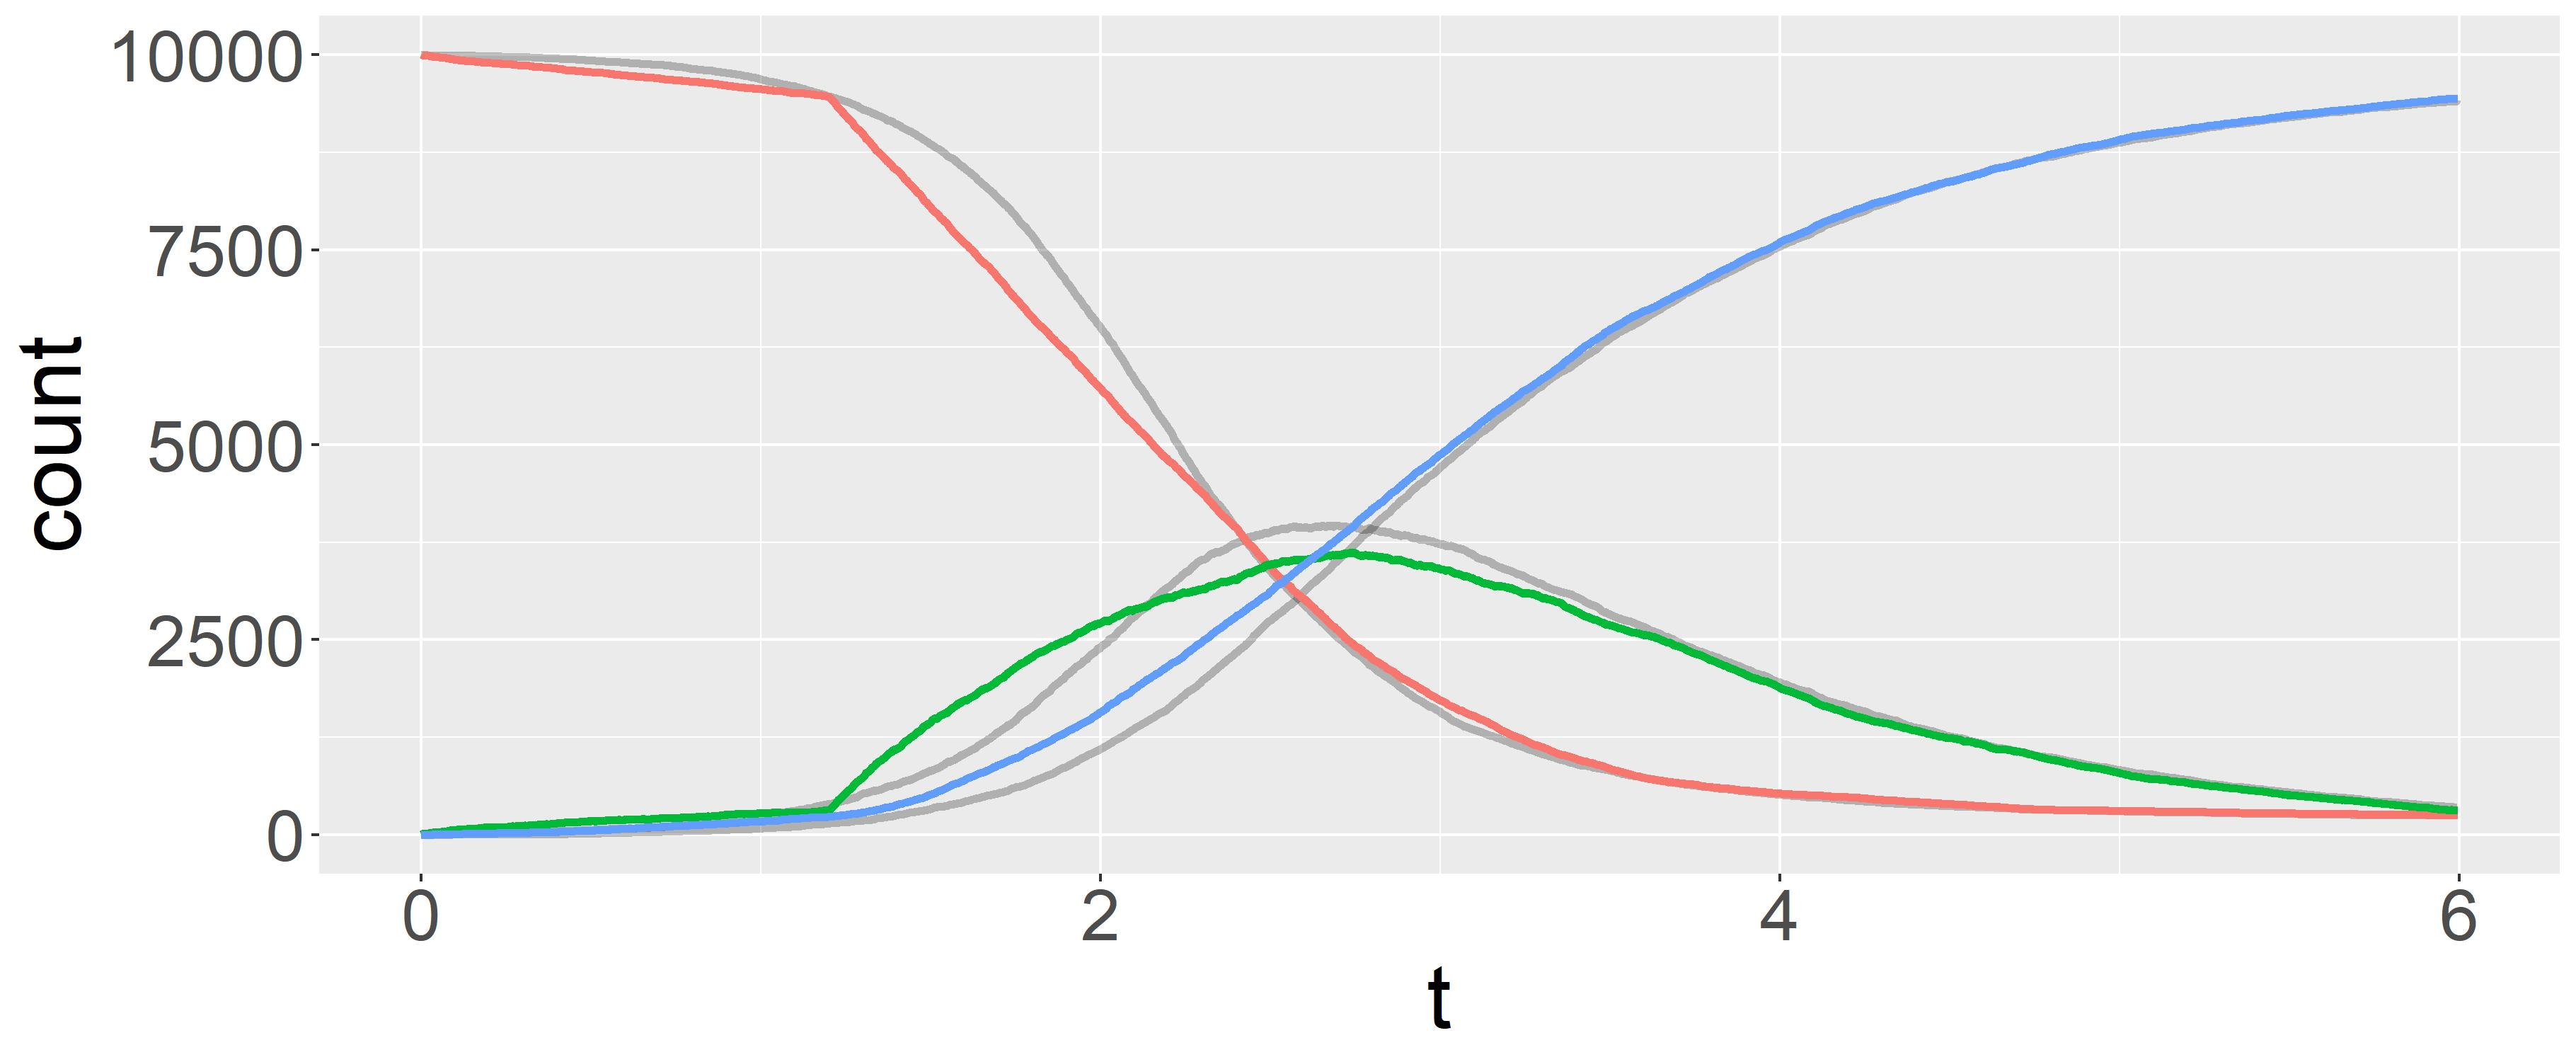
\includegraphics[width=\textwidth]{E2_K5.jpg}
			\caption{PD-SIR process ($K = 5$)}
			\label{fig:comparison_RD_SIR_K5}
		\end{subfigure}
		\hfill
		\begin{subfigure}[b]{0.49\textwidth}
			\centering
			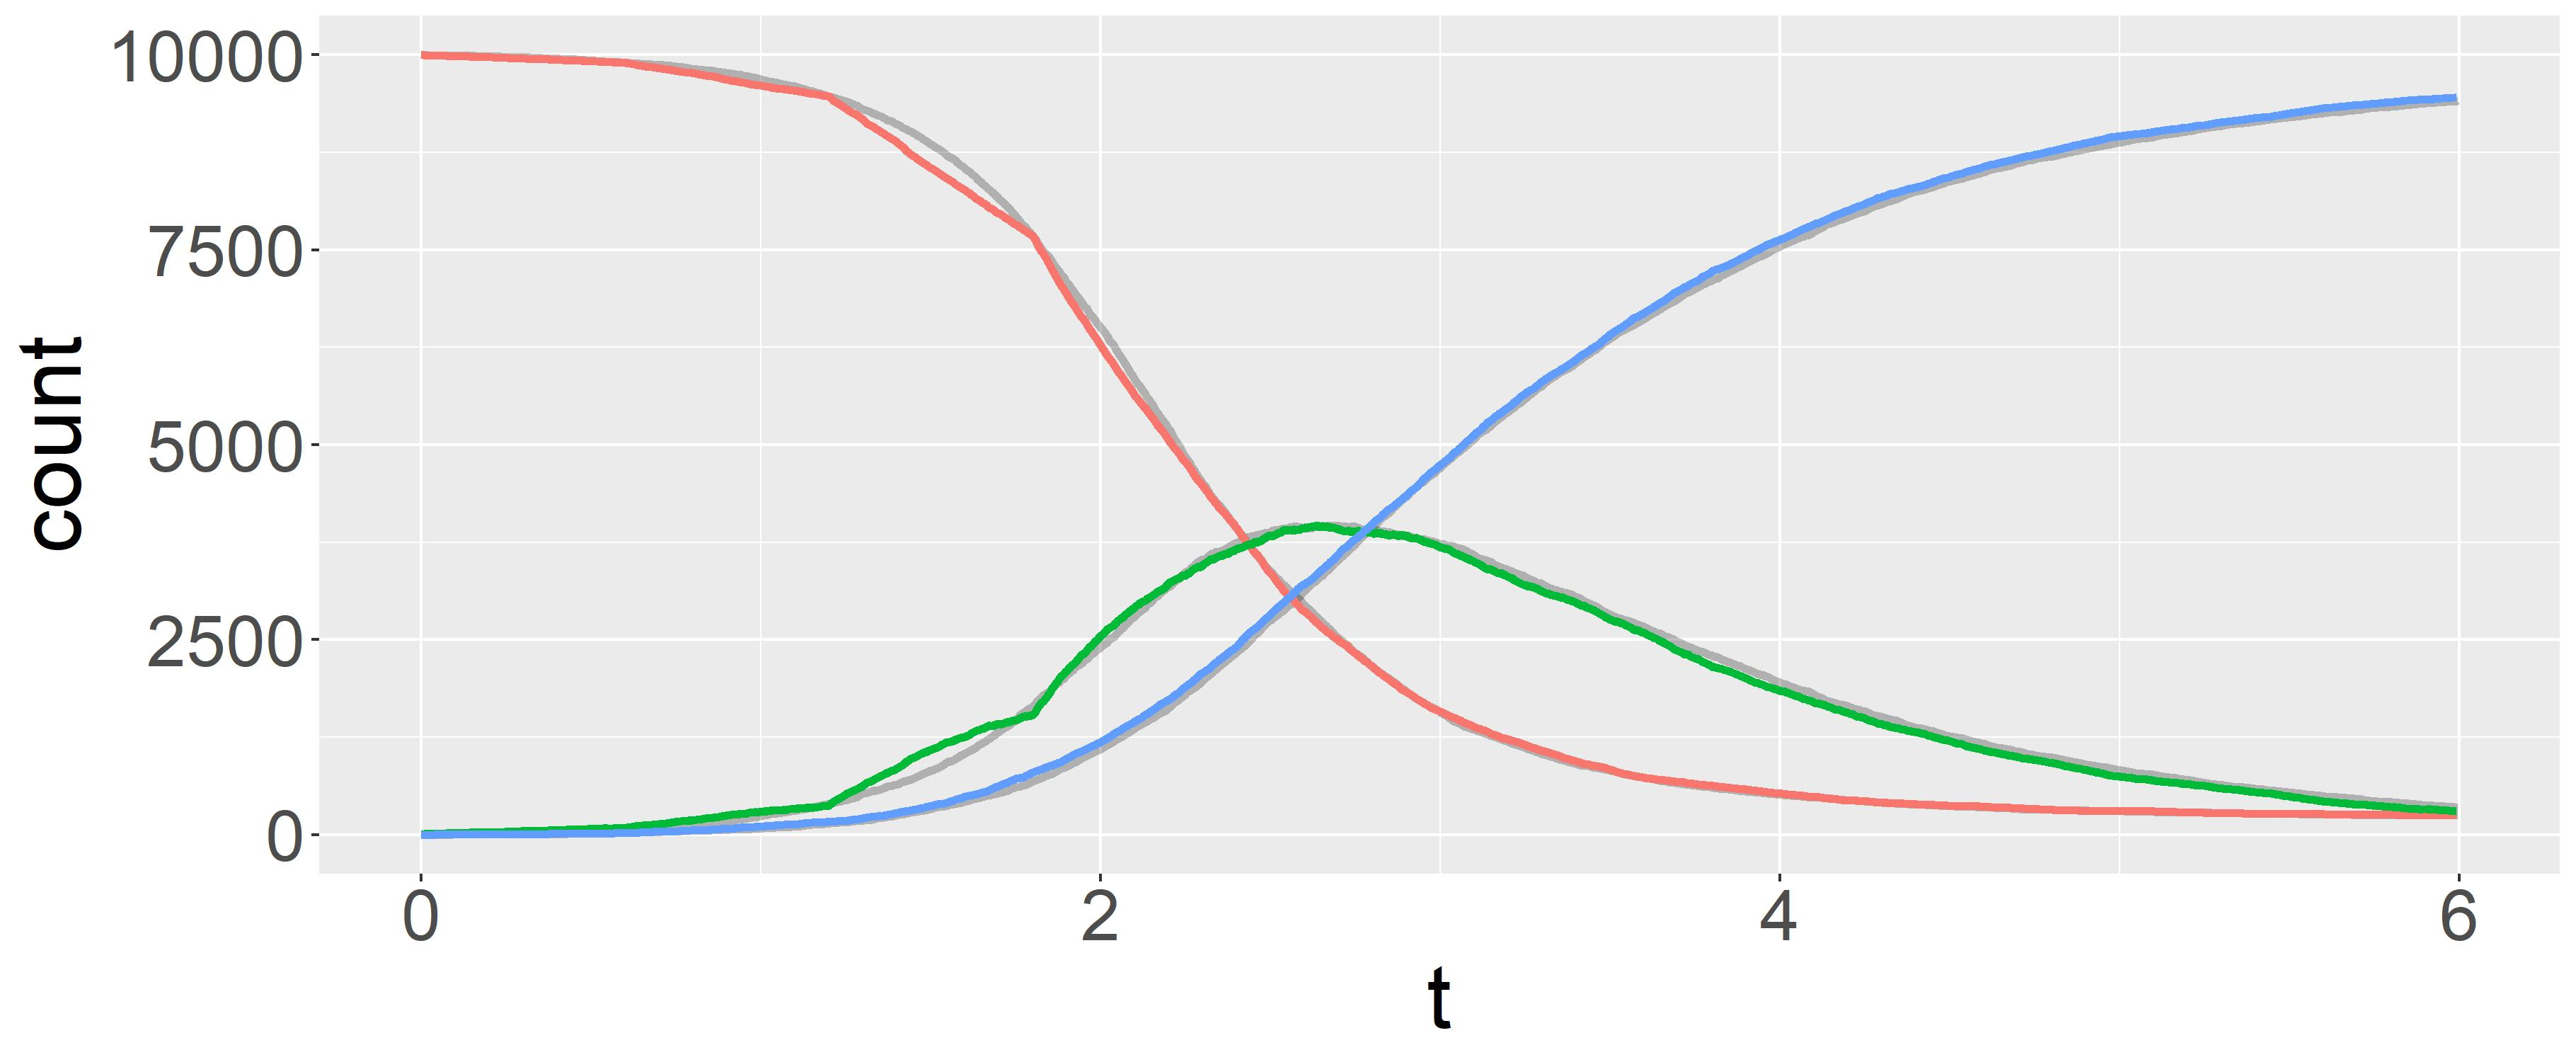
\includegraphics[width=\textwidth]{E2_K10.jpg}
			\caption{PD-SIR process ($K = 10$)}
			\label{fig:comparison_RD_SIR_K10}
		\end{subfigure}
		\\
		\begin{subfigure}[b]{0.49\textwidth}
			\centering
			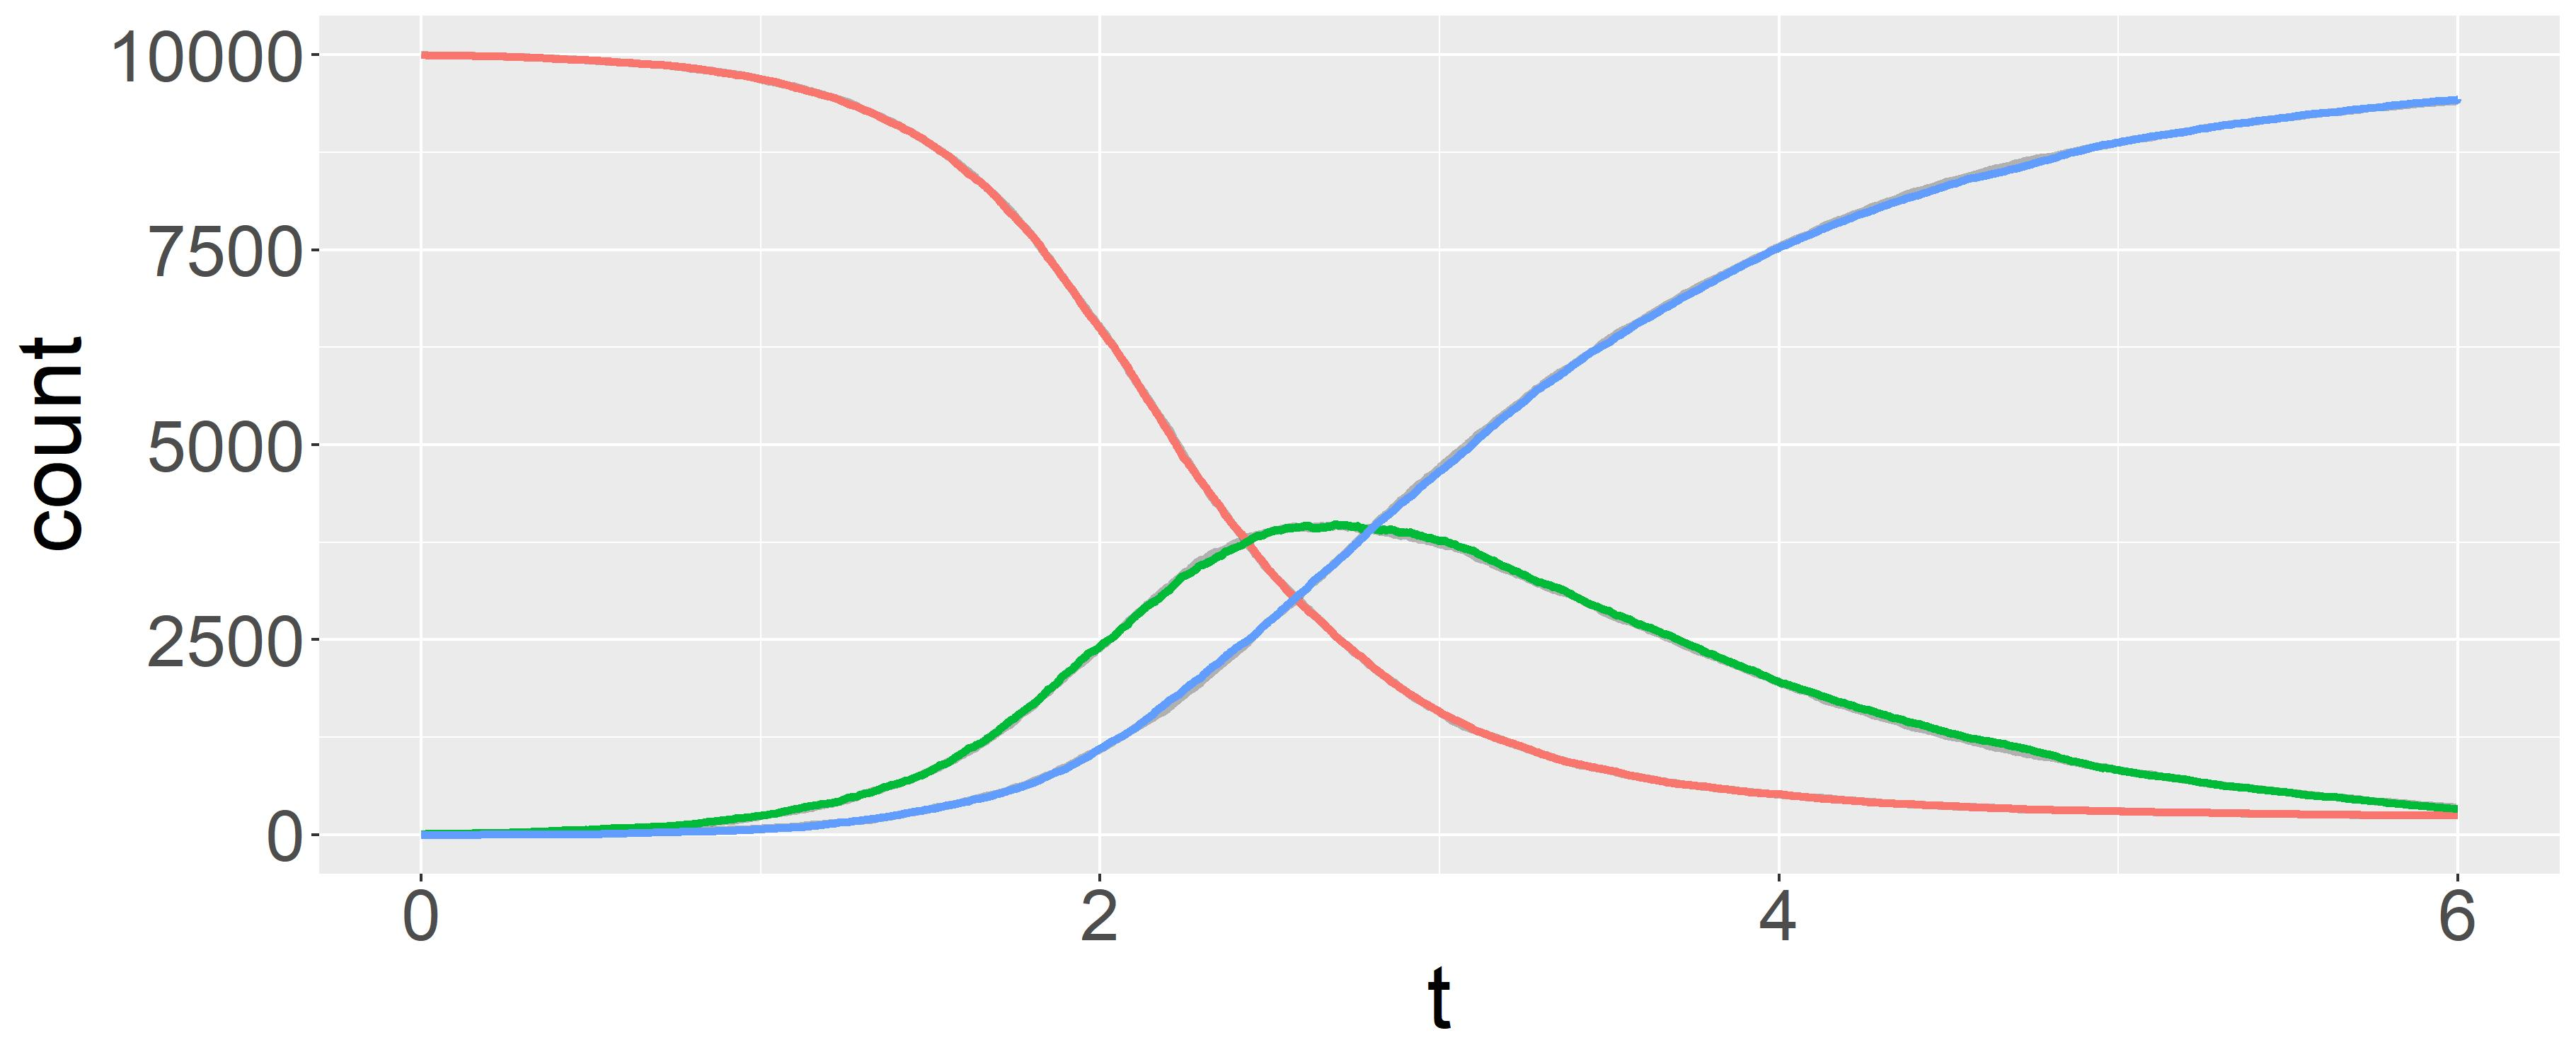
\includegraphics[width=\textwidth]{E2_K50.jpg}
			\caption{PD-SIR process ($K = 50$)}
			\label{fig:comparison_RD_SIR_K50}
		\end{subfigure}
		\hfill
		\begin{subfigure}[b]{0.49\textwidth}
			\centering
			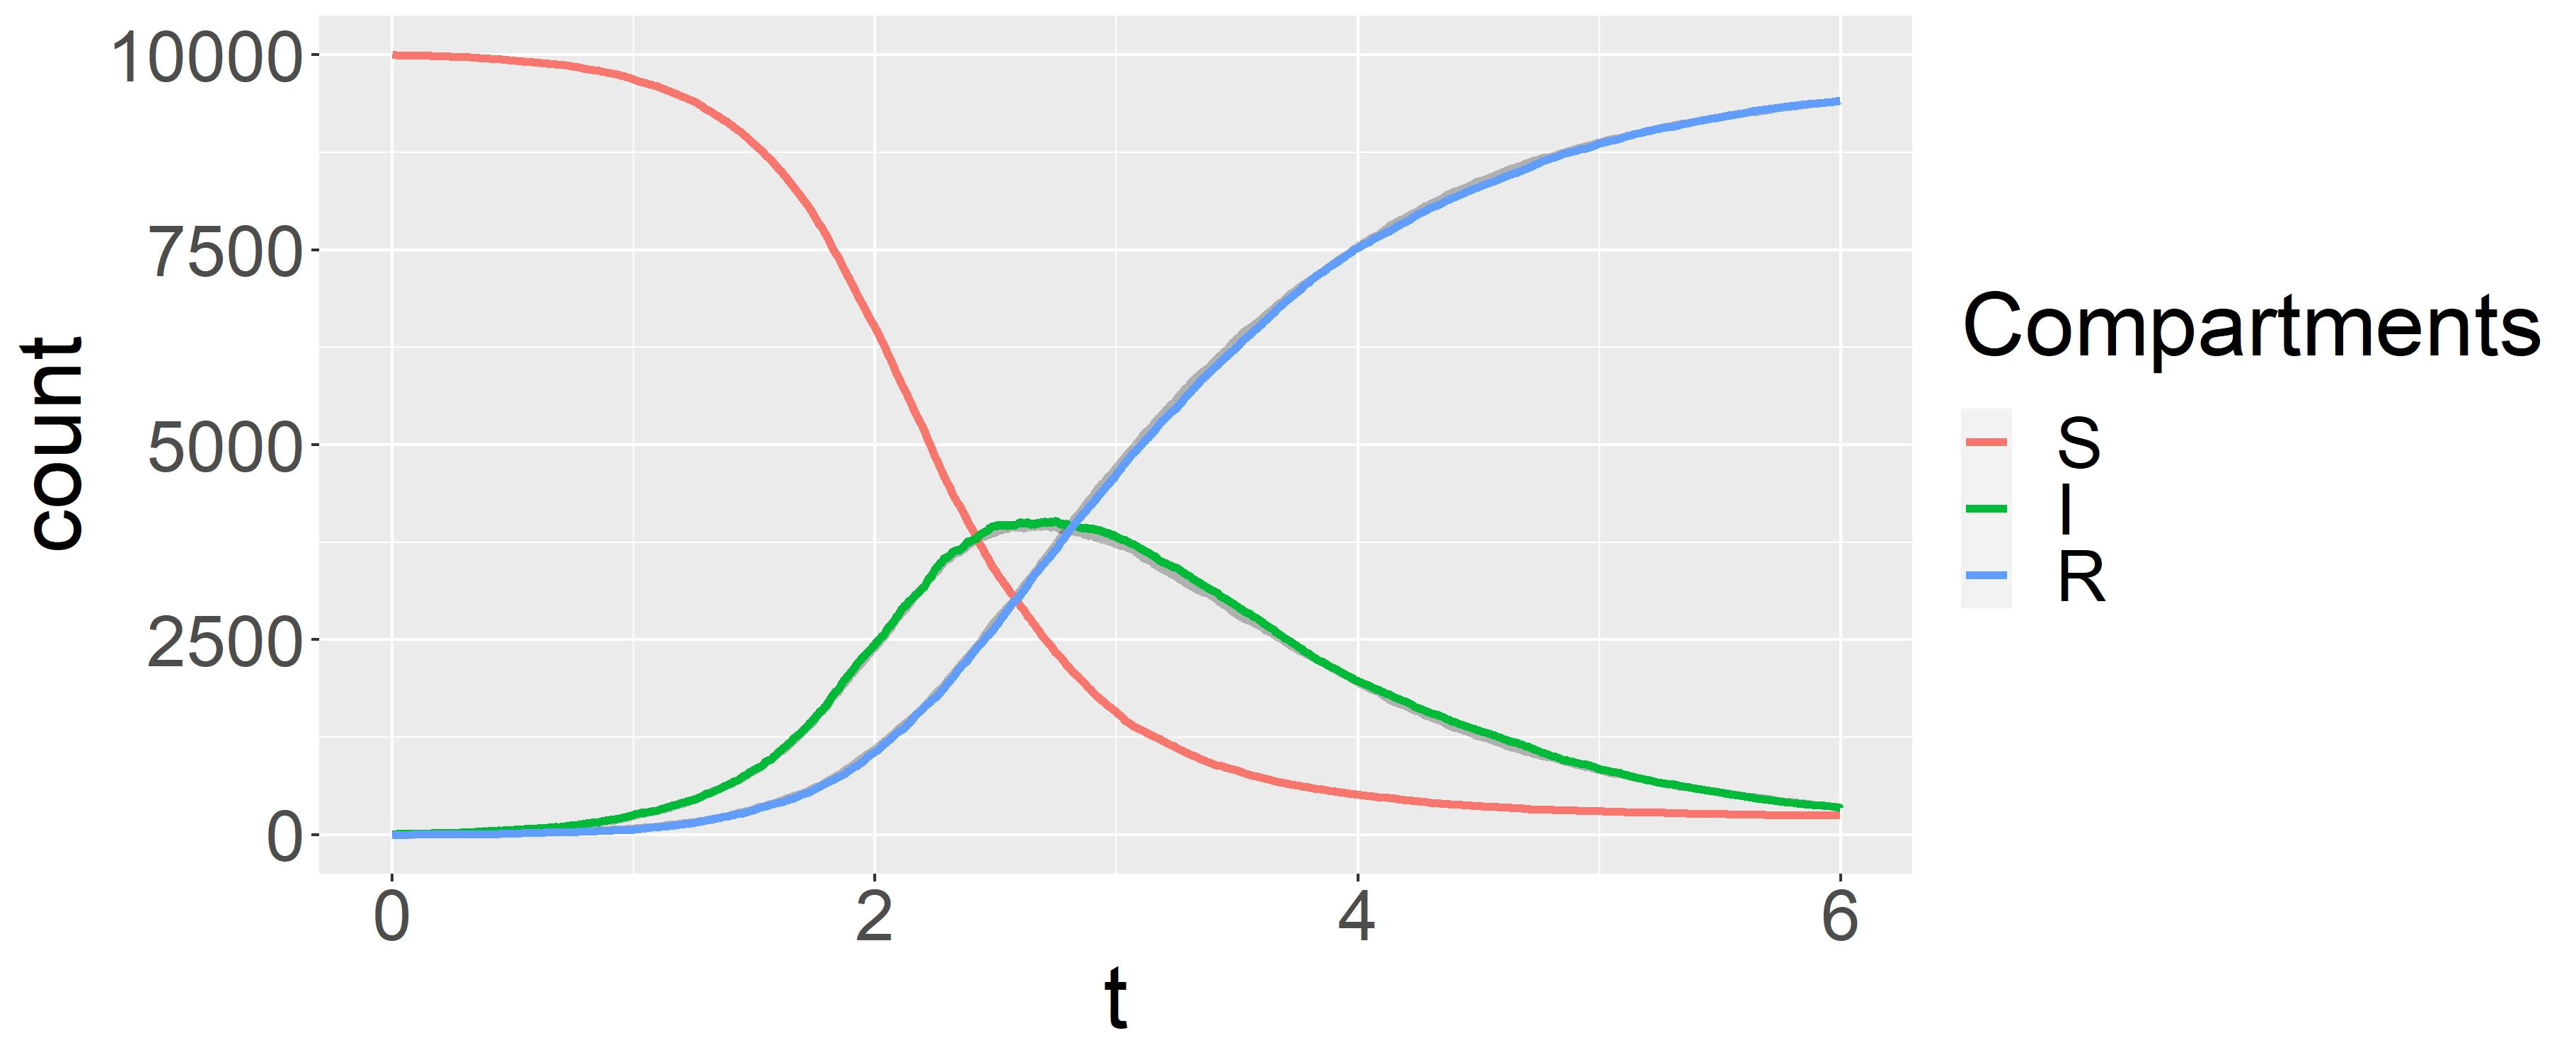
\includegraphics[width=\textwidth]{E2_K1000.jpg}
			\caption{PD-SIR process ($K = 1000$)}
			\label{fig:comparison_RD_SIR_K1000}
		\end{subfigure}
		\caption{Trajectories of the compartments $S$, $I$ and $R$ in a SIR (in colors) and PD-SIR processes (in grey) with the same infection incidence data $T_{1:K}$.}
		\label{fig:comparison}
	\end{figure}
	
	
	\section{Performance on simulated and real epidemic data}
	\label{sec:per}
	
	\subsection{Simulation Study}
	\label{sec:sim}
	%Outline: setup; results: posterior mean, credible interval, frequentist coverage, run time, ACF, acceptance rate; table; figure: traceplot, ACF; tuning: update proportion v. acceptance rate; compare with others methods e.g. chain binomial, exact proposal.
	
	% 1. convergence in medium-size population
	% 2. rho
	% 3. nominal coverage should be 95%.
	% 4. distribution of estimate for PD-SIR (unbiased) vs. LNA (biased)
	% explain why not compare chain binomial, particle filtering (forward simulation). 
			
	In this section, the convergence properties of the DA-MCMC algorithm are examined with a simulation study. Each data set in this study is simulated from the stochastic SIR model and the prior distributions on the parameters $\beta$ and $\gamma$ are independent weakly informative gamma distribution with scale and shape parameters set to $0.01$ (see Equation \ref{eq:pri}).
	
	First, the mixing property of the Markov chain is assessed in a medium-size population of $S(0)=1,000$ initially susceptible and $I(0)=10$ initially infectious individuals. The parameters are $(\beta, \gamma) = (0.003, 1)$ and the process is observed until time $t_{end} = 6$ when the pandemic has completed most of its course but is not over yet (see Figure \ref{fig:long}, where $I(t_{end}) = 55$). The numbers of infections in $K = 10$ intervals of equal length are observed and correspond to $T_{1:K} = (40, 111, 193, 259, 178, 93, 29, 19, 9, 6)$. The Markov chain is run for $100,000$ iterations from the initial values $(\beta^{(1)}, \gamma^{(1)}) = (0.0003, 0.1) = (\beta/10, \gamma/10)$ and the event times of $202$ ($\rho = 0.2$) individuals are updated in the augmented data in each Metropolis-Hastings step. The algorithm took less than $5$ minutes to complete on a personal laptop. Figure \ref{fig:traceplot} shows the traceplots of the parameters $\beta$ and $\gamma$, the log likelihood and the basic reproduction number $R_0 = S(0) \beta / \gamma$, which corresponds to the average number of secondary infections caused by an infectious individual at the beginning of the outbreak. We observe that the Markov chain quickly migrates from the low density region of the space where it started to a high density region where it mixes relatively well. The acceptance rate of the latent spaces proposed in the Metropolis-Hastings step is $0.11$.
	Excluding the first $10,000$ iterations of the Markov chain as a burn-in, the posterior means of $\beta$, $\gamma$ and $R_0$ are respectively $0.00304$, $0.995$ and $3.07$.
	
	% TODO: Results: convergence (R statistic, Geweke), credible intervals.
	% TODO: Tables: posterior means, credible intervals, effective sample size.
			
	% TODO: frequentist coverage for 3 different observation schedules
	
	% TODO: Geweke
	
	\begin{figure}
		\centering
		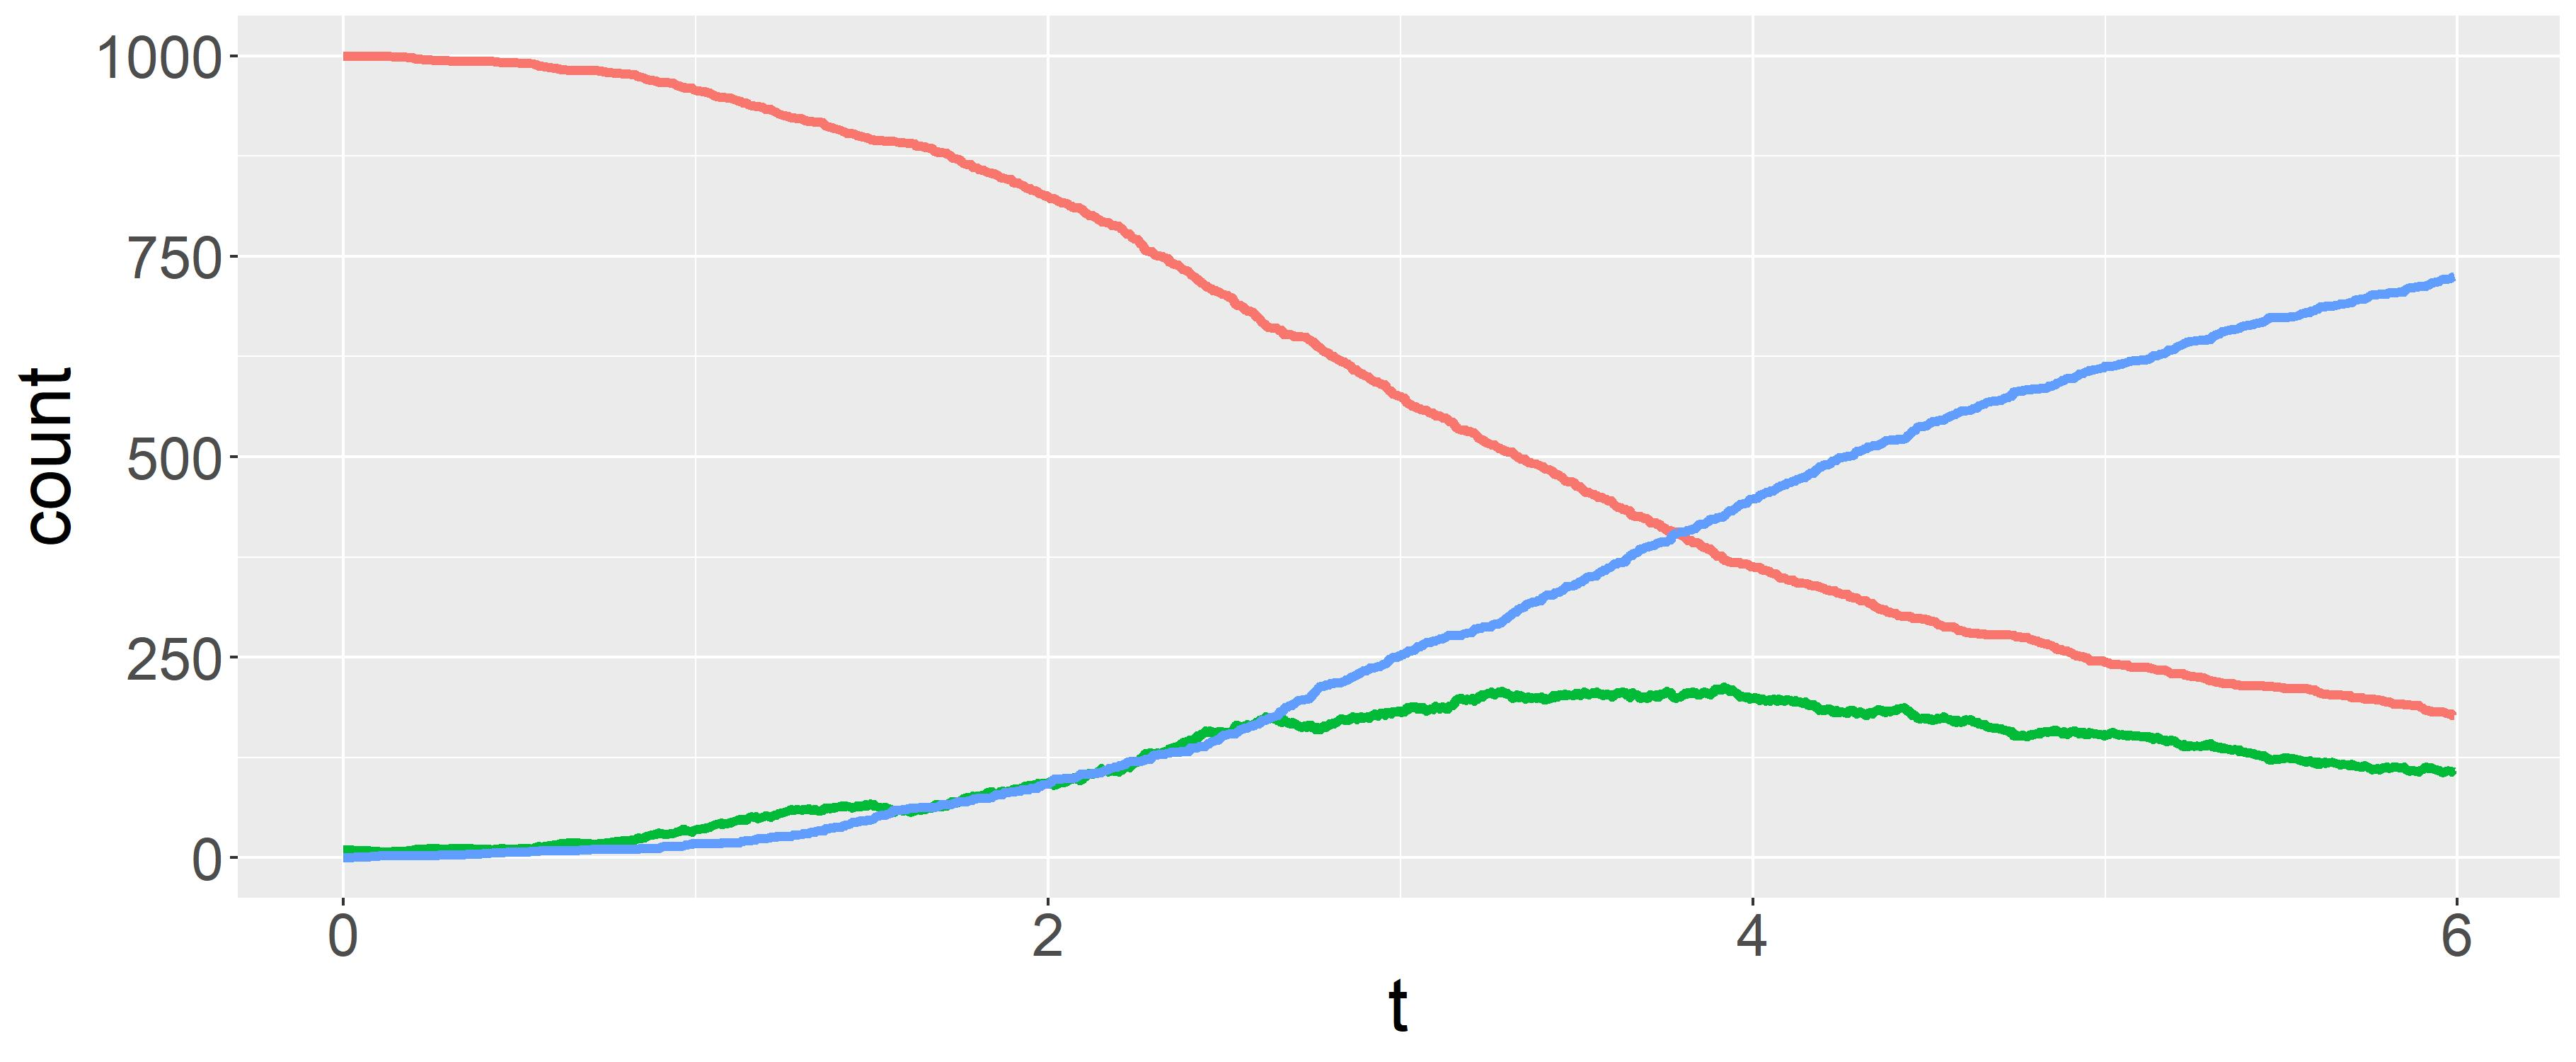
\includegraphics[scale = 0.3]{E1_trajectories.jpg}
		\caption{Trajectories of the $S$, $I$ and $R$ compartments of a SIR process for a medium-size population ($S_0 = 1,000$).}
		\label{fig:long}
	\end{figure}
	
	\begin{figure}
		\centering
		\begin{subfigure}[b]{0.41\textwidth}
			\centering
			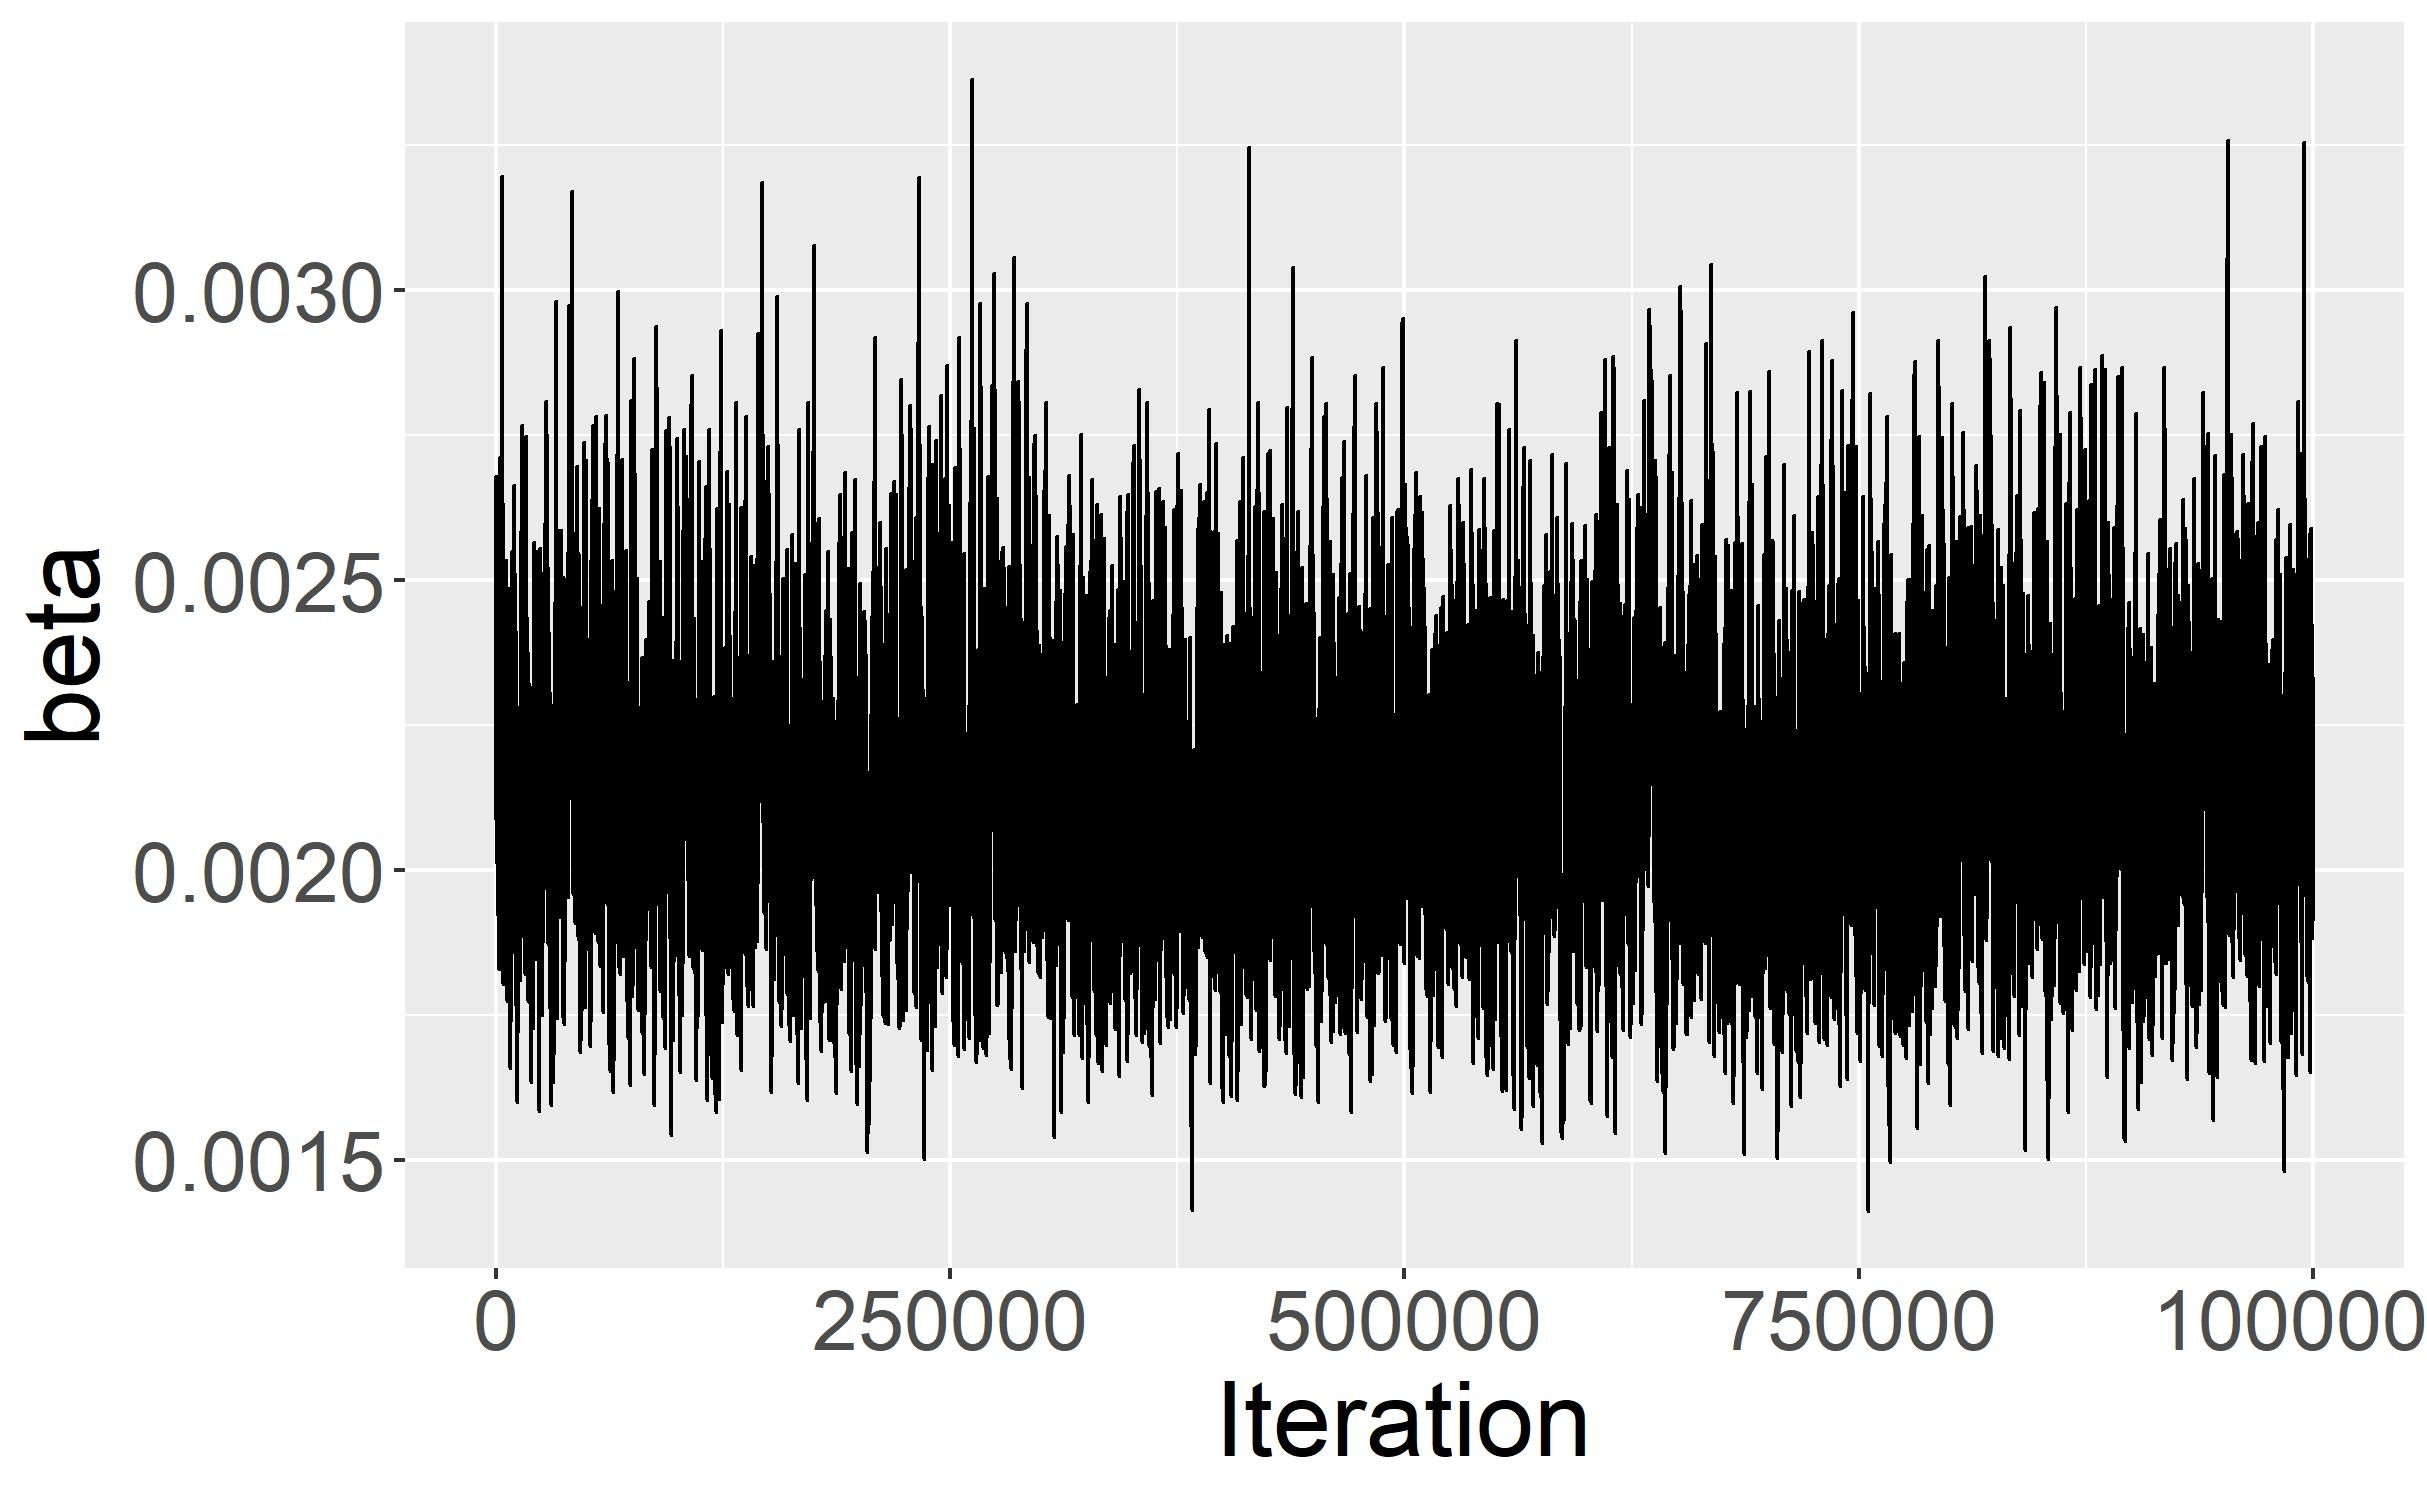
\includegraphics[width=\textwidth]{E1_no_burn_beta_tp.jpg}
			\caption{$\beta$}
			\label{fig:traceplot_beta}
		\end{subfigure}
		\hfill
		\begin{subfigure}[b]{0.41\textwidth}
			\centering
			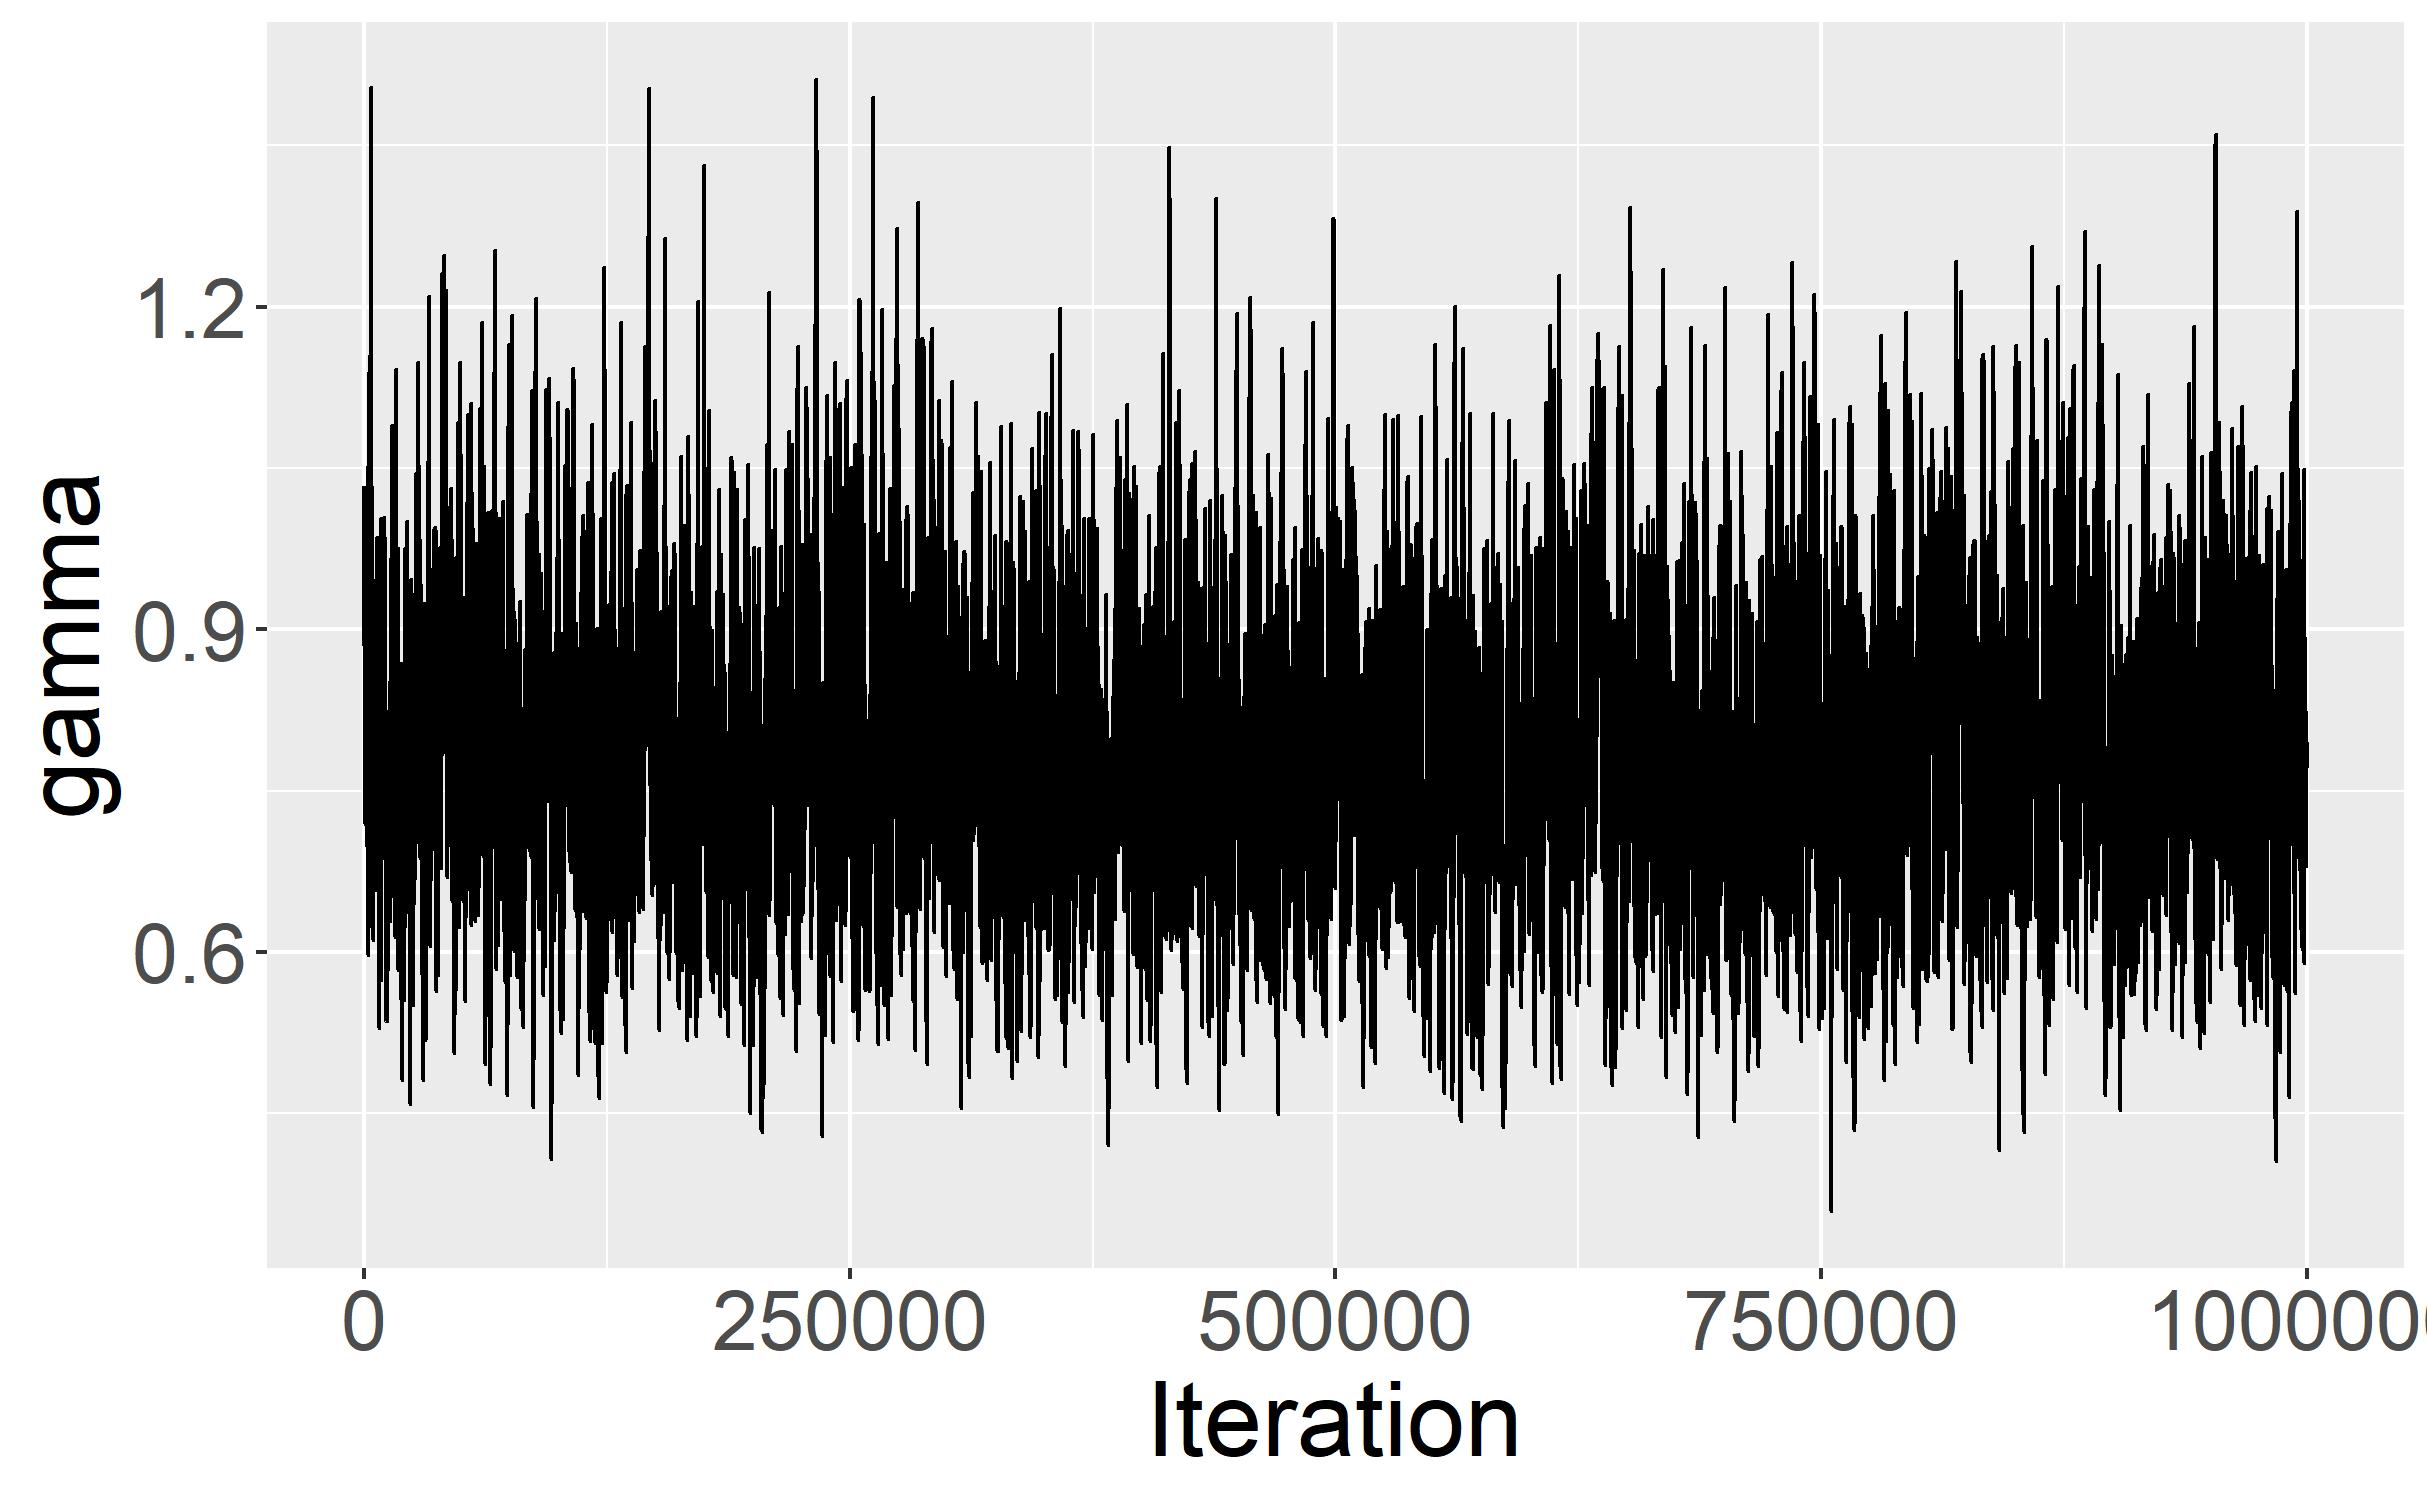
\includegraphics[width=\textwidth]{E1_no_burn_gamma_tp.jpg}
			\caption{$\gamma$}
			\label{fig:traceplot_gamma}
		\end{subfigure}
		\\
		\begin{subfigure}[b]{0.41\textwidth}
			\centering
			\includegraphics[width=\textwidth]{E1_no_burn_loglik_tp.jpg}
			\caption{Log likelihood}
			\label{fig:traceplot_loglik}
		\end{subfigure}
		\hfill
		\begin{subfigure}[b]{0.41\textwidth}
			\centering
			\includegraphics[width=\textwidth]{E1_no_burn_R0_tp.jpg}
			\caption{$R_0$}
			\label{fig:traceplot_R0}
		\end{subfigure}
		\caption{Traceplots of the Markov chain (including burn-in).}
		\label{fig:traceplot}
	\end{figure}
	
	Second, the impact of the tuning parameter $\rho$ on the performance of the MCMC algorithm is evaluated. In particular, we examine the acceptance rate of the Metropolis-Hastings step, the total run time of the algorithm and the auto-correlation function of the parameters.
	Three SIR processes with different population sizes $S(0) = (10^2, 10^3, 10^4)$ are simulated. We set $I(0) =10$, $\gamma=1$, $t_{end} = 3$ and $K = 50$ for all simulations and $\beta = (0.001, 0.01, 0.1)$ respectively for the three different population sizes. These values for $\beta$ ensure that the three processes have comparable dynamics. For each process, the DA-MCMC algorithm is run for $50,000$ iterations with different values of $\rho = (10^{-4}, 10^{-3}, 10^{-2}, 10^{-1}, 0.5, 1)$. The algorithm is run only if there is at least one event time updated per iteration, that is, if $\rho(S_0+I_0)>1$.
	Figure \ref{fig:accept} presents the acceptance rate across the range of $\rho$.  We observe that the acceptance rate decreases as the number of event times updated per iteration and the population size increase.
	Figure \ref{fig:run_time} shows the run time of the MCMC algorithm for these simulations. The run time increases with the population size and with $\rho$.
	Finally, Figure \ref{fig:acf} shows the effect of $\rho$ on the auto correlation function for the parameter $\beta$ for the medium-size population process ($S(0) = 1,000$) for three values of $\rho$. We observe that updating half of the augmented data per iteration yields the lowest auto-correlation function across the values of $\rho$ considered. This suggests that, in this setting, updating the entire latent space in the Metropolis-Hastings step results in too many rejections while updating a tenth or less prevents the chain from efficiently exploring the latent space.
	
	\begin{figure}
		\centering
		\includegraphics[scale = 0.4]{E3_1000_ESS_sec_R0.jpg}
		\caption{Acceptance rate of the proposed latent spaces in the Metropolis-Hastings step of the MCMC algorithm across different population sizes and values for $\rho$.}
		\label{fig:ESS_sec}
	\end{figure}			
				
							
	\begin{figure}
		\centering	
\centering
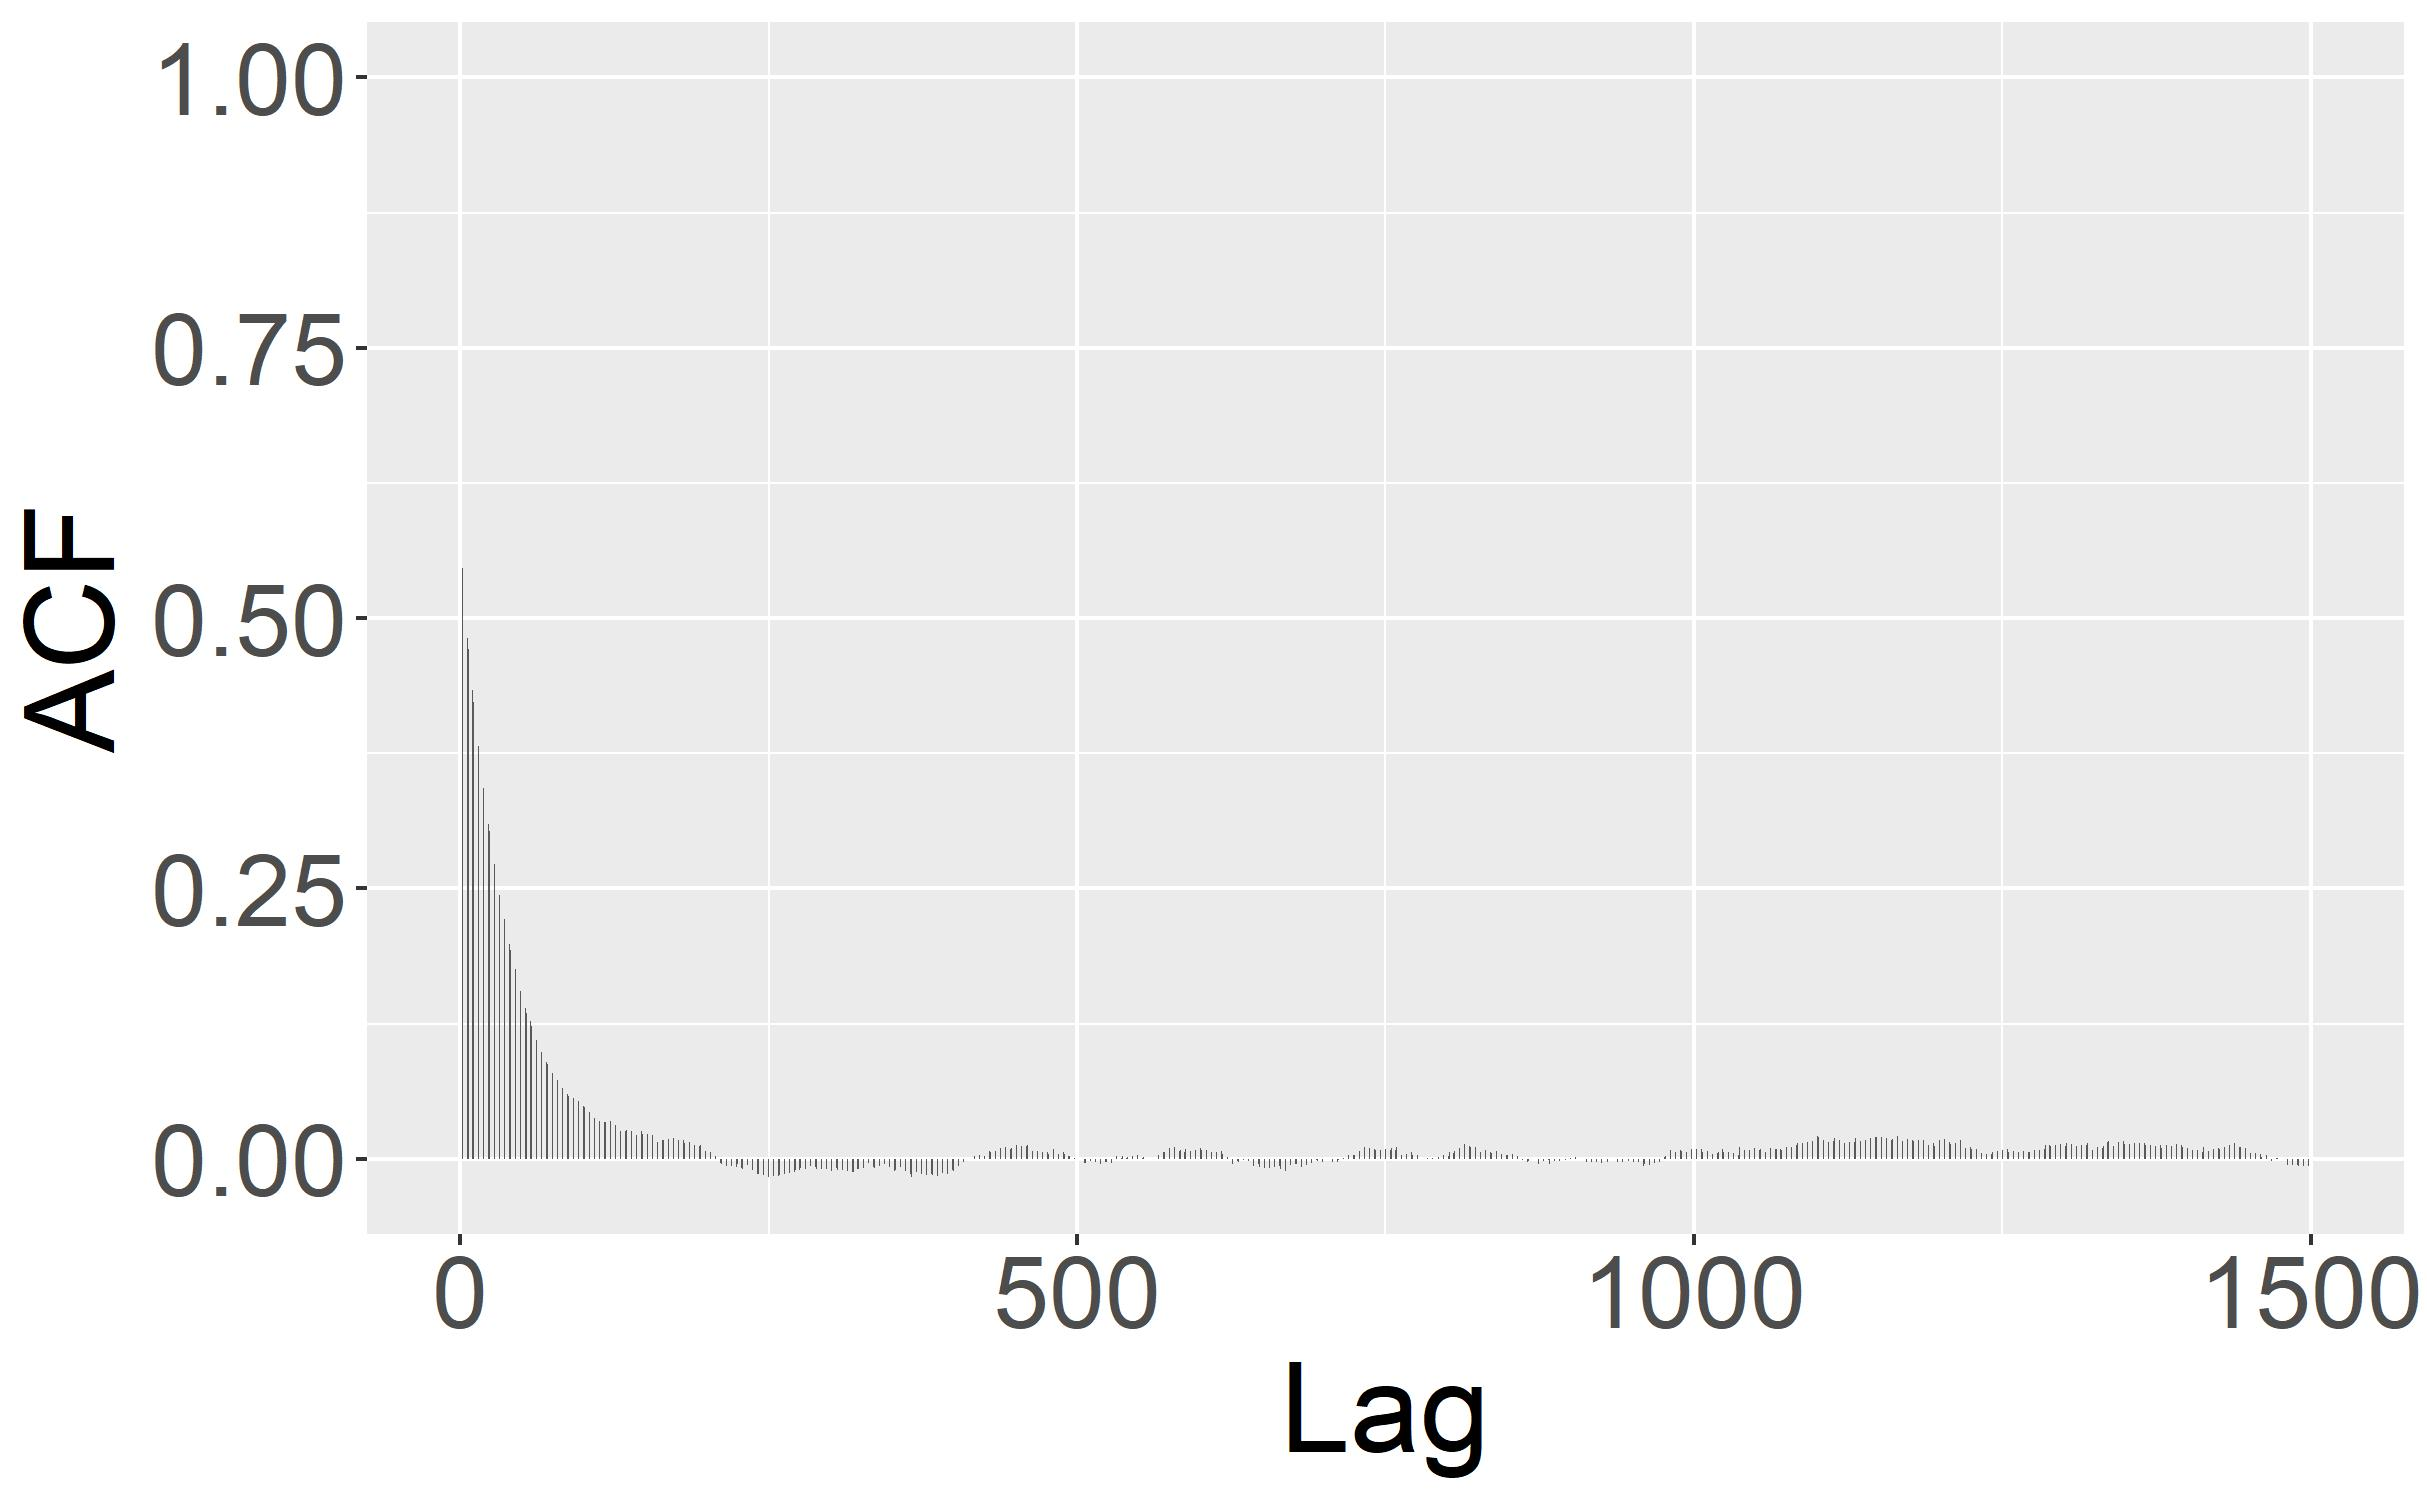
\includegraphics[width=\textwidth]{E1_burn_R0_acf.jpg}
\caption{$\rho = 0.1$}
\label{fig:acf}
	\end{figure}

	%Figures: acceptance rate v. proportion of updates (see Neal, Roberts A case study in non-centering -- table 1 p.319).
		
	\subsection{Ebola Outbreak in Gu\'eck\'edou, Guinea}
	\label{sec:ebo}
	%Outline: background; setup; results; table; figure
	
	We now turn to a case study concerning the Ebola outbreak in Western Africa.
	Between the end of $2013$ and $2015$, Guinea, along with several neighboring countries, experienced the largest outbreak of the Ebola virus disease in history. The virus, which has a fatality rate of $70\%$, was responsible for the death of almost $2,000$ people in Guinea alone during the outbreak.
	The outbreak is believed to have originated in the Gu\'eck\'edou prefecture of Guinea at the end of November $2013$ \cite{Baize.2014}. Weekly infection incidence counts are available for each prefecture for the $73$ weeks between the end of December $2013$ and May $2015$.
	We fit the stochastic SIR model to these incidence counts for the Gu\'eck\'edou prefecture using the MCMC algorithm proposed in this article.
	For simplicity, we assume that the population of the prefecture forms a closed population, that the model's parameters remained constant throughout the outbreak and that the reported infections counts are exact. Applying our MCMC algorithm to stochastic epidemic models where these assumptions are relaxed is the subject of ongoing research.
	The \textit{effective} population size is set to $n = 150,000$, roughly half of the total population in $2014$. Note that as long as the number of infections is small compared to the total population size, the exact population size does not need to be known to estimate the parameters of the model. Furthermore, since the first documented infection occurred late November, one month before the first reported incidence count \cite{Baize.2014}, the number of infectious individuals at the beginning of the observation period is set to $I(0) = 10$, with the units of time corresponding to ``days" in the analysis.
		
	The Markov chain is run for $50,000$ iterations and the event times of $10\%$ of the individuals are updated each iteration. The initial values of the parameters are set to $(\beta^{(1)}, \gamma^{(1)}) = (10^{-7}, 0.05)$ and the conjugate distributions in Equation \ref{eq:pri} are used as priors with $a_{\beta} = b_{\beta} = a_{\gamma} = b_{\gamma} = 0.01$ to make them weakly informative. Even for such a large population, the total run time of the algorithm was less than $100$ minutes on a personal laptop.
	The Metropolis-Hastings step for the latent space proposals achieves a healthy $22.1\%$ acceptance rate, and the first $10,000$ iterations of the Markov chain are discarded as a burn-in.
	Figure \ref{fig:ebola} shows the joint posterior distributions of $(\beta, \gamma)$, whose posterior means are respectively $1.06 * 10^{-6}$ and $0.109$, as well as the marginal distribution of the basic reproduction number $R_0$. This value for $\gamma$ indicates that people remain infectious for around $9$ days on average, which is consistent with existing literature. As noted by numerous authors, conditionally on partially observed data, the parameters $\beta$ and $\gamma$ appear positively correlated. The posterior distribution of $R_0$ is unimodal, relatively symmetric, and centered around $1$. A basic reproduction number close to $1$ is consistent with an outbreak that lasted several months without infecting the majority of the population.
	
	\begin{figure}
		\centering
		\begin{subfigure}[b]{0.45\textwidth}
			\centering
			\includegraphics[width=\textwidth]{E5_burn_HPD.jpeg}
			\caption{Joint posterior density of $\theta = (\beta, \gamma)$. The $50\%$ and $90\%$ confidence regions are shown.}
			\label{fig:density_joint}
		\end{subfigure}
		\hfill
		\begin{subfigure}[b]{0.49\textwidth}
			\centering
			\includegraphics[width=\textwidth]{E5_burn_R0_hist.jpg}
			\caption{Posterior density of $R_0$.}
			\label{fig:density_R0}
		\end{subfigure}
		\caption{Posterior densities of parameters of interest (excluding burn-in of $10,000$ iterations).}
		\label{fig:ebola}
	\end{figure}
	
	\section{Discussion and Conclusion}
	\label{sec:dis}
	The method proposed in this article enables the classical Metropolis-Hastings algorithm to be an efficient method to conduct full posterior inference of the stochastic SIR model given only incidence data. Existing attempts using Markov chain Monte Carlo either mix poorly or do not scale to populations of more than a few hundred individuals, while methods relying on forward simulation are limited to moderate-sized outbreaks and may suffer from degeneracy issues on a case-by-case basis depending on the amount of missing data. 	Moreover, the simplifying assumptions in \cite{Fintzi.2020} or the approximate-Bayesian-computation framework of \cite{McKinley.2018}, which compromise targeting the exact posterior for computational reasons, generate biased estimates that may lead to spurious conclusions. Instead, our data-augmented algorithm enables fast and exact inference, even for large outbreaks, and leverages a well-studied, transparent MCMC framework. %Most existing inferential methods for epidemic stochastic models are only applicable to prevalence data. To our knowledge, our algorithm is the first that permits exact Bayesian inference given incidence data.
			
	Central to the success of the DA-MCMC algorithm is an efficient proposal scheme that swiftly explores the latent space of epidemic paths that are compatible with the observed data. The PD-SIR process possesses three features that yield such an efficient algorithm. First, generating a PD-SIR process is extremely fast; it only requires the simulation of truncated exponential distributions, which can efficiently be realized via the inverse-CDF method. Moreover, the individual infection rates are only updated $K$ times, as opposed to after each event as in the SIR model. Second, generating a PD-SIR process that is constrained to be compatible with the observed incidence data can be done at no additional cost; in contrast, generating a SIR process compatible with the observed data would be prohibitively slow \cite{Hobolth.2009}. Third, the dynamics of the PD-SIR process closely resemble those of the SIR process: the removal dynamics are identical and, for short resetting intervals, the infection dynamics are also very similar in the two processes.
	
	The first two features make the algorithm extremely fast. While existing data-augmented MCMC algorithms have only be applied to populations of a few hundred of individuals, the analysis of the Ebola outbreak in Gu\'eck\'edou shows that our algorithm can be applied to populations of up to $150,000$ individuals, generating tens of thousands of posterior samples in a reasonable amount of time.	
	The latter feature of the PD-SIR process enables the algorithm to update a large portion of the augmented data in each iteration while maintaining a healthy acceptance rate. As a result, the Markov chain makes large jumps in the latent space and has very good mixing properties. In contrast, existing DA-MCMC algorithms keep most of the latent space fixed across iterations \cite{Gibson.1998, ONeill.1999, Fintzi.2017} and their Markov chains therefore mix much more slowly.
	
	The algorithm possesses a tuning parameter $\rho$ that determines the portion of the augmented data being updated each iteration. Larger values for $\rho$ enable the chain to make larger steps in the latent space but can result in a low acceptance rate, while smaller values of $\rho$ result in a higher acceptance rate but constrain the chain to make small jumps. Depending on the size of the population, different values of the tuning parameter are optimal. To find a value that optimizes the mixing properties of the chain, one can use several short runs of the algorithm with different values for $\rho$ and select the value that yields the lowest auto-correlation function (ACF). Since the run time of the algorithm increases with $\rho$, one could also look at the effective sample size per unit of time. For instance, for populations of a few hundred individuals, we observed that updating the entire augmented data ($\rho=1$) yields the lowest ACF. In this case, the current and proposed augmented data are independent conditionally on the current value of the parameters.
		
	The DA-MCMC algorithm proposed in this article is specific to the stochastic SIR model, which is arguably a simplistic representation of the spread of disease. The model relies on assumptions such as perfect reporting, constant infection rates, homogeneously mixing population and exponentially-distributed infectious periods. In future work, we will present applications of our DA-MCMC algorithm to processes where these assumptions are relaxed. In particular, we are considering extensions to epidemic models with under-reporting, a varying infection rate, stratified populations and non-Markovian dynamics, as well as the general stochastic SIR model of \cite{Severo.1969}.
			
			
	\appendix
	
	\section{Distribution of Death Times in Linear Death Process}
	\label{app:ldp}
	Theorem \ref{theo:ldp} was first proved by \cite{Neuts.1971}. Since this is a result that has rarely been mentioned in the literature, we provide a proof in this appendix from (cite Ross textbook).
	
	Consider a linear pure death process with $n$ particles and individual death rate $\mu$.
	Let $T_i$ be the time of the $i$th death. Then $W_1 = T_1 \sim \Exp(n\mu)$ and $W_i = T_i - T_{i-1} \sim \Exp((n-1)\mu)$ independently. Let $N$ be the number of deaths by time $t$. Then, 
	\begin{align*}
		& f(T_1 = t_1, \dots, T_N = t_N | N) \\
		& \propto f(T_1 = t_1, \dots, T_N = t_N, T_{N+1} > t) 1\{T_N < t\}\\
		& \propto f(W_1 = t_1, W_2 = t_2 - t_1, \dots, W_N = t_N - t_{N-1}, W_{N+1} > t - t_N) 1\{T_N < t\}\\
		& \propto \exp\{-n\mu t_1\} \exp\{-(n-1)\mu(t_2-t_1)\}\dots \exp\{-(n-N)\mu(t - t_N)\} 1\{T_N < t\}\\
		& \propto \exp\{-\mu t_1\}\exp\{-\mu t_2\} \dots \exp\{-\mu t_N\} 1\{T_N < t\}
	\end{align*}
which corresponds to the kernels of independent exponential distribution truncated above by $t$.

	
	\section{Uniform Ergodicity}
	\label{app:uni}
	We show that the state space $\chi = \chi_{\theta}\times\chi_{\z}$ of the Markov chain $\{(\theta, \z)^{(i)}\}_i$ is a small set for the transition kernel $P$, that is, there exists a probability measure $\nu$ on the $\sigma$-algebra $\sigma(\chi)$ such that
	$$\beta \nu(.) \le P^m(x,.), \forall x\in \chi.$$
	for some constants $m \ge 1$ and $\beta > 0$.
	By Proposition 2 in \cite{Tierney.1994}, this implies that the Markov chain $\{(\theta, \z)^{(i)}\}_i$ is uniformly ergodic and therefore satisfies
	$$
	\Vert P^n(x,.)-\pi(.)\Vert_{TV} \le M r^n
	$$
	for some finite $M$ and positive constant $r<1$, where $\Vert \mu \Vert_{TV}$ denotes the total variation norm of the measure $\mu$.
	
	The following three lemmas are used to show this result.
	
	
	% Gamma 1
	\begin{lemma}
		\label{pro:ga1}
		Let $Ga(x;a,b)$ denote the density of a gamma distribution with shape $a$ and rate $b$ evaluated at $x$. Then
		\begin{equation}
			\label{eq:ga1}
			\inf_{0\le \beta\le B} Ga(x;a,b+\beta) = 
			\begin{cases}
				Ga(x;a,b), & x<x_a^* \\ Ga(x;a,b+B), & x\ge x_a^*
			\end{cases}
		\end{equation}	
		where $x_a^*=\frac{a}{B}\log\left( 1+\frac{B}{b}\right) $. Moreover,
		\begin{equation}
			\label{eq:ga2}
			\inf_{0\le \alpha\le A} Ga(x;a+\alpha,b) = 
			\begin{cases}
				Ga(x;a,b), & x>x_b^* \\ Ga(x;a+A,b), & x\le x_b^*
			\end{cases}
		\end{equation}
		where $x_b^*=\frac{1}{b}\left[ \frac{\Gamma(a+A)}{\Gamma(a)}\right]^{1/A} $.
	\end{lemma}
	
	\begin{proof}
		Equation \ref{eq:ga1} is proven in Jones, Hobert (2004). For Equation \ref{eq:ga2}, note that $x_b^*$ is the only positive solution to $Ga(x;a,b) = Ga(x;a+A,b)$. Now, for all $0<x\le x_b^*$ and all $0\le\alpha\le A$, we have
		\begin{align*}
			\frac{Ga(x;a+A,b)}{Ga(x;a+\alpha,b)}
			& = b^{A-\alpha}x^{A-\alpha} \frac{\Gamma(a+\alpha)}{\Gamma(a+A)} \\
			& \le b^{A-\alpha}\left(\frac{1}{b}\left[ \frac{\Gamma(a+A)}{\Gamma(a)}\right]^{1/A} \right)^{A-\alpha} \frac{\Gamma(a+\alpha)}{\Gamma(a+A)} \\
			& = \left[ \frac{\Gamma(a+A)}{\Gamma(a)}\right]^{(A-\alpha)/A} \frac{\Gamma(a+\alpha)}{\Gamma(a+A)} \\
			& = \left( \frac{\Gamma_{a,a+A}}{\Gamma_{a+\alpha, a+A}}\right)^{A-\alpha} \\
			& \le 1,
		\end{align*}
		where $\Gamma_{d,e} = \left( \frac{\Gamma(e)}{\Gamma(d)} \right)^{\frac{1}{e-d}}$ is a geometric average,
		and where the last inequality holds because $\Gamma_{a,a+A}\le\Gamma_{a+\alpha, a+A}$.
		The case $x>x_b^*$ can be shown similarly.
	\end{proof}

\begin{figure}
	\centering
	\begin{subfigure}[b]{0.45\textwidth}
		\centering
		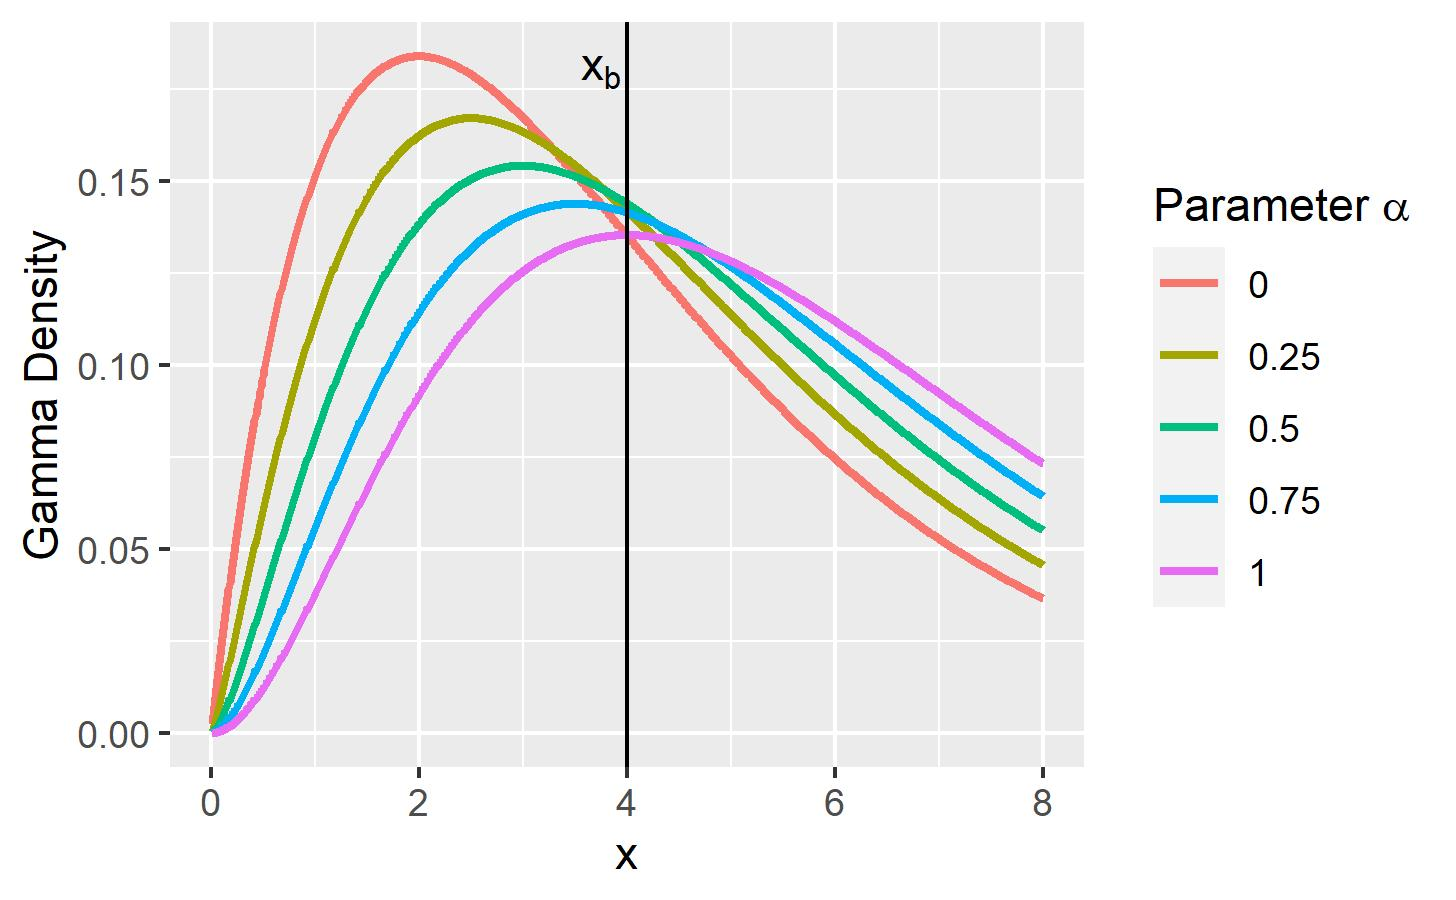
\includegraphics[width=\textwidth]{gamma_minorization_1a.jpg}
		\caption{$\alpha \in [0, 1]$, $\beta=0$}
		\label{fig:gam1a}
	\end{subfigure}
	\hfill
	\begin{subfigure}[b]{0.49\textwidth}
		\centering
		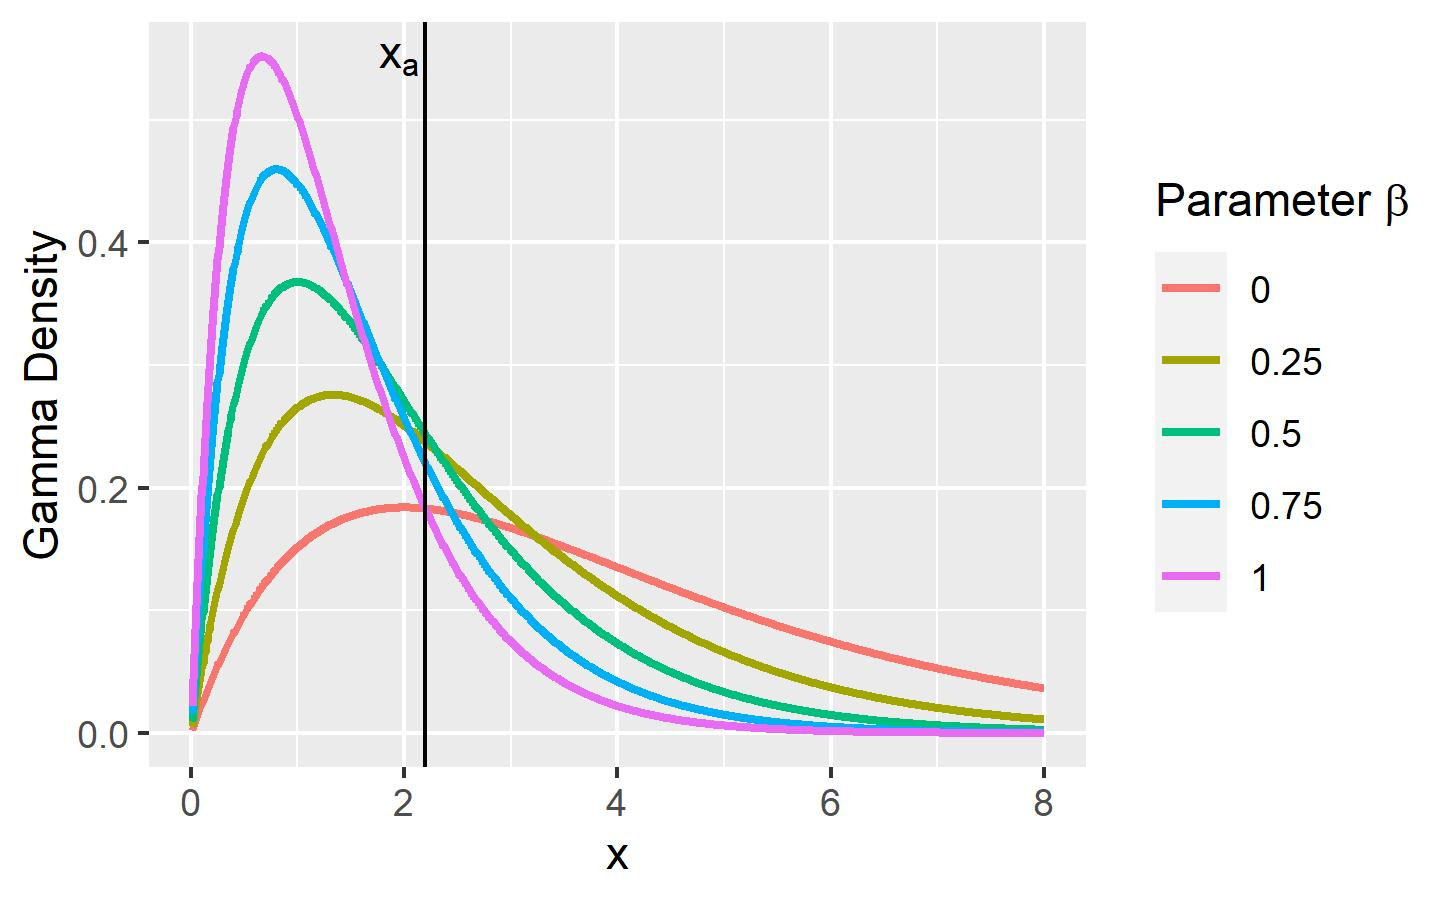
\includegraphics[width=\textwidth]{gamma_minorization_1b.jpg}
		\caption{$\alpha = 0$, $\beta \in [0, 1]$}
		\label{fig:gam1b}
	\end{subfigure}
	\caption{Example of minorization of the density of a gamma distribution $Ga(2+\alpha, 0.5+\beta)$ for $\alpha$ and $\beta$ separately.}
	\label{fig:gam1}
\end{figure}


% Gamma 2
Proposition \ref{pro:ga1} can be used to minorize a density of the form
\begin{equation}
	\label{eq:ga}
	Ga(x;a+\alpha,b+\beta) = \frac{(b+\beta)^{a+\alpha}}{\Gamma(a+\alpha)}x^{a+A-1}\exp\{-x(b+B)\}, \quad 0\le\alpha\le A, 0\le\beta\le B.
\end{equation}
over $\alpha$ and $\beta$ for each value of $x$. We can show the following.
\begin{lemma}	
	\label{pro:ga2}
	For a fix $x>0$, the density $Ga(x;a+\alpha,b+\beta)$ is minimized by $(\alpha, \beta) \in \{(A, 0), (0, B)\}$, the minimizing set of values depending on $x$. In particular,	
	$$\inf_{\begin{aligned}
			0\le \alpha\le A \\ 0\le \beta\le B
	\end{aligned}}Ga(x;a+\alpha,b+\beta) = 
	\begin{cases}
		Ga(x;a+A,b)                     , & x<x_a         \text{ or } x<x_{a+A}^* \vee x_b^*\\
		Ga(x;a,b+B)                     , & x_{a+A}^* < x \text{ or } x_a^* \wedge x_{b+B}^* < x\\
		\min\{Ga(x;a+A,b), Ga(x;a,b+B)\}, & x_a^* \wedge x_b^*\le x < x_{a+A}^* \vee x_{b+B}^*\\
	\end{cases}$$
\end{lemma}

\begin{proof}
	Given $x>0$, \ref{eq:ga1} shows that for a fixed $\alpha$, $\beta \in \{0, B\}$ is the minimizer of \ref{eq:ga}, and \ref{eq:ga2} shows that for a fixed $\beta$, $\alpha \in \{0, A\}$ is the minimizer of \ref{eq:ga}. This implies that for a fixed $x>0$, \ref{eq:ga} is minimized by $(\alpha, \beta) \in \{(0,0), (A, 0), (0, B), (A,B)\}$.
	
	A case-by-case analysis of the nine possibilities
	$$(x<x_a^*; x_a^*<x<x_{a+A}^*; x_{a+A}^* < x )\times(x<x_{b+B}^*; x_{b+B}^*<x<x_b^*; x_b^* < x)$$
	is presented in Table \ref{tab:ga9} and shows that it is sufficient to consider $(\alpha, \beta) \in \{(A, 0), (0, B)\}$.
	
	\begin{table}[H]
		\centering
		\begin{tabular}{l|c c c}
			& $x<x_a^*$  & $x_a^*\le x<x_{a+A}^*$ & $x_{a+A}^* < x$ \\ \hline
			$x<x_b^*$              & $(a+A, b)$ & $(a+A, b)$             &                 \\
			$x_b^*\le x<x_{b+B}^*$ & $(a+A, b)$ &  ad hoc                & $(a, b+B)$      \\
			$x_{b+B}^* < x$        &            & $(a, b+B)$             & $(a, b+B)$
		\end{tabular}
		\caption{Values of $(\alpha, \beta)$ that minimize $Ga(x;a+\alpha,b+\beta)$ for different values $x$.}
		\label{tab:ga9}
	\end{table}
	
	The two empty entries in Table \ref{tab:ga9} correspond to impossible configurations. Indeed, $x_b^* > x_a^*$ and $x_{a+A}^* > x_{b+B}^*$ for all $a, A, b, B$ since
	$$
	\frac{x_b^*}{x_a^*} = \dfrac{\left(\frac{\Gamma(a+A)}{\Gamma(a)}\right)^{1/A} b^{-1} }{a B^{-1} \log\left( 1+B/b\right)} = \dfrac{\left(\frac{\Gamma(a+A)}{\Gamma(a)}\right)^{1/A}}{a} \dfrac{B/b}{\log\left( 1+B/b\right)} = \dfrac{\Gamma_{a,a+A}}{a} \dfrac{B/b}{\log\left( 1+B/b\right)} \ge 1
	$$
	and
	$$
	\frac{x_{b+B}^*}{x_{a+A}^*} = \dfrac{\left(\frac{\Gamma(a+A)}{\Gamma(a)}\right)^{1/A} (b+B)^{-1} }{(a+A) B^{-1} \log\left( 1+B/b\right)} = \dfrac{\Gamma_{a,a+A}}{a+A} \dfrac{B}{b+B} \dfrac{1}{\log\left( 1+B/b\right)} \le 1
	$$
	where the inequalities hold since $a \le \Gamma_{a,a+A} \le a+A$ and $\dfrac{y}{\log\left( 1+y\right)}\le1$.
		
	If $x_a^* \wedge x_{b+B}^*\le x < x_{a+A}^* \vee x_{b}^*$, which corresponds to the middle entry of the center column in Table \ref{tab:ga9}, then one needs to directly check which set of values in $\{(0,0), (A, 0), (0, B), (A,B)\}$ minimizes Equation \ref{eq:ga}. In fact, it is sufficient to consider only $\{(A,0), (0, B)\}$ since
	$$Ga(x, a+A, b) \le \begin{cases}
		Ga(x;a,b), & x < x_b^* \\
		Ga(x;a+A,b+B), & x < x_{a+A}^* 
	\end{cases}$$
	and
	$$Ga(x, a, b+B) \le \begin{cases}
		Ga(x;a,b), & x > x_a^* \\
		Ga(x;a+A,b+B), & x > x_{b+B}^* 
	\end{cases}$$
\end{proof}

							
\begin{figure}	
	\centering
	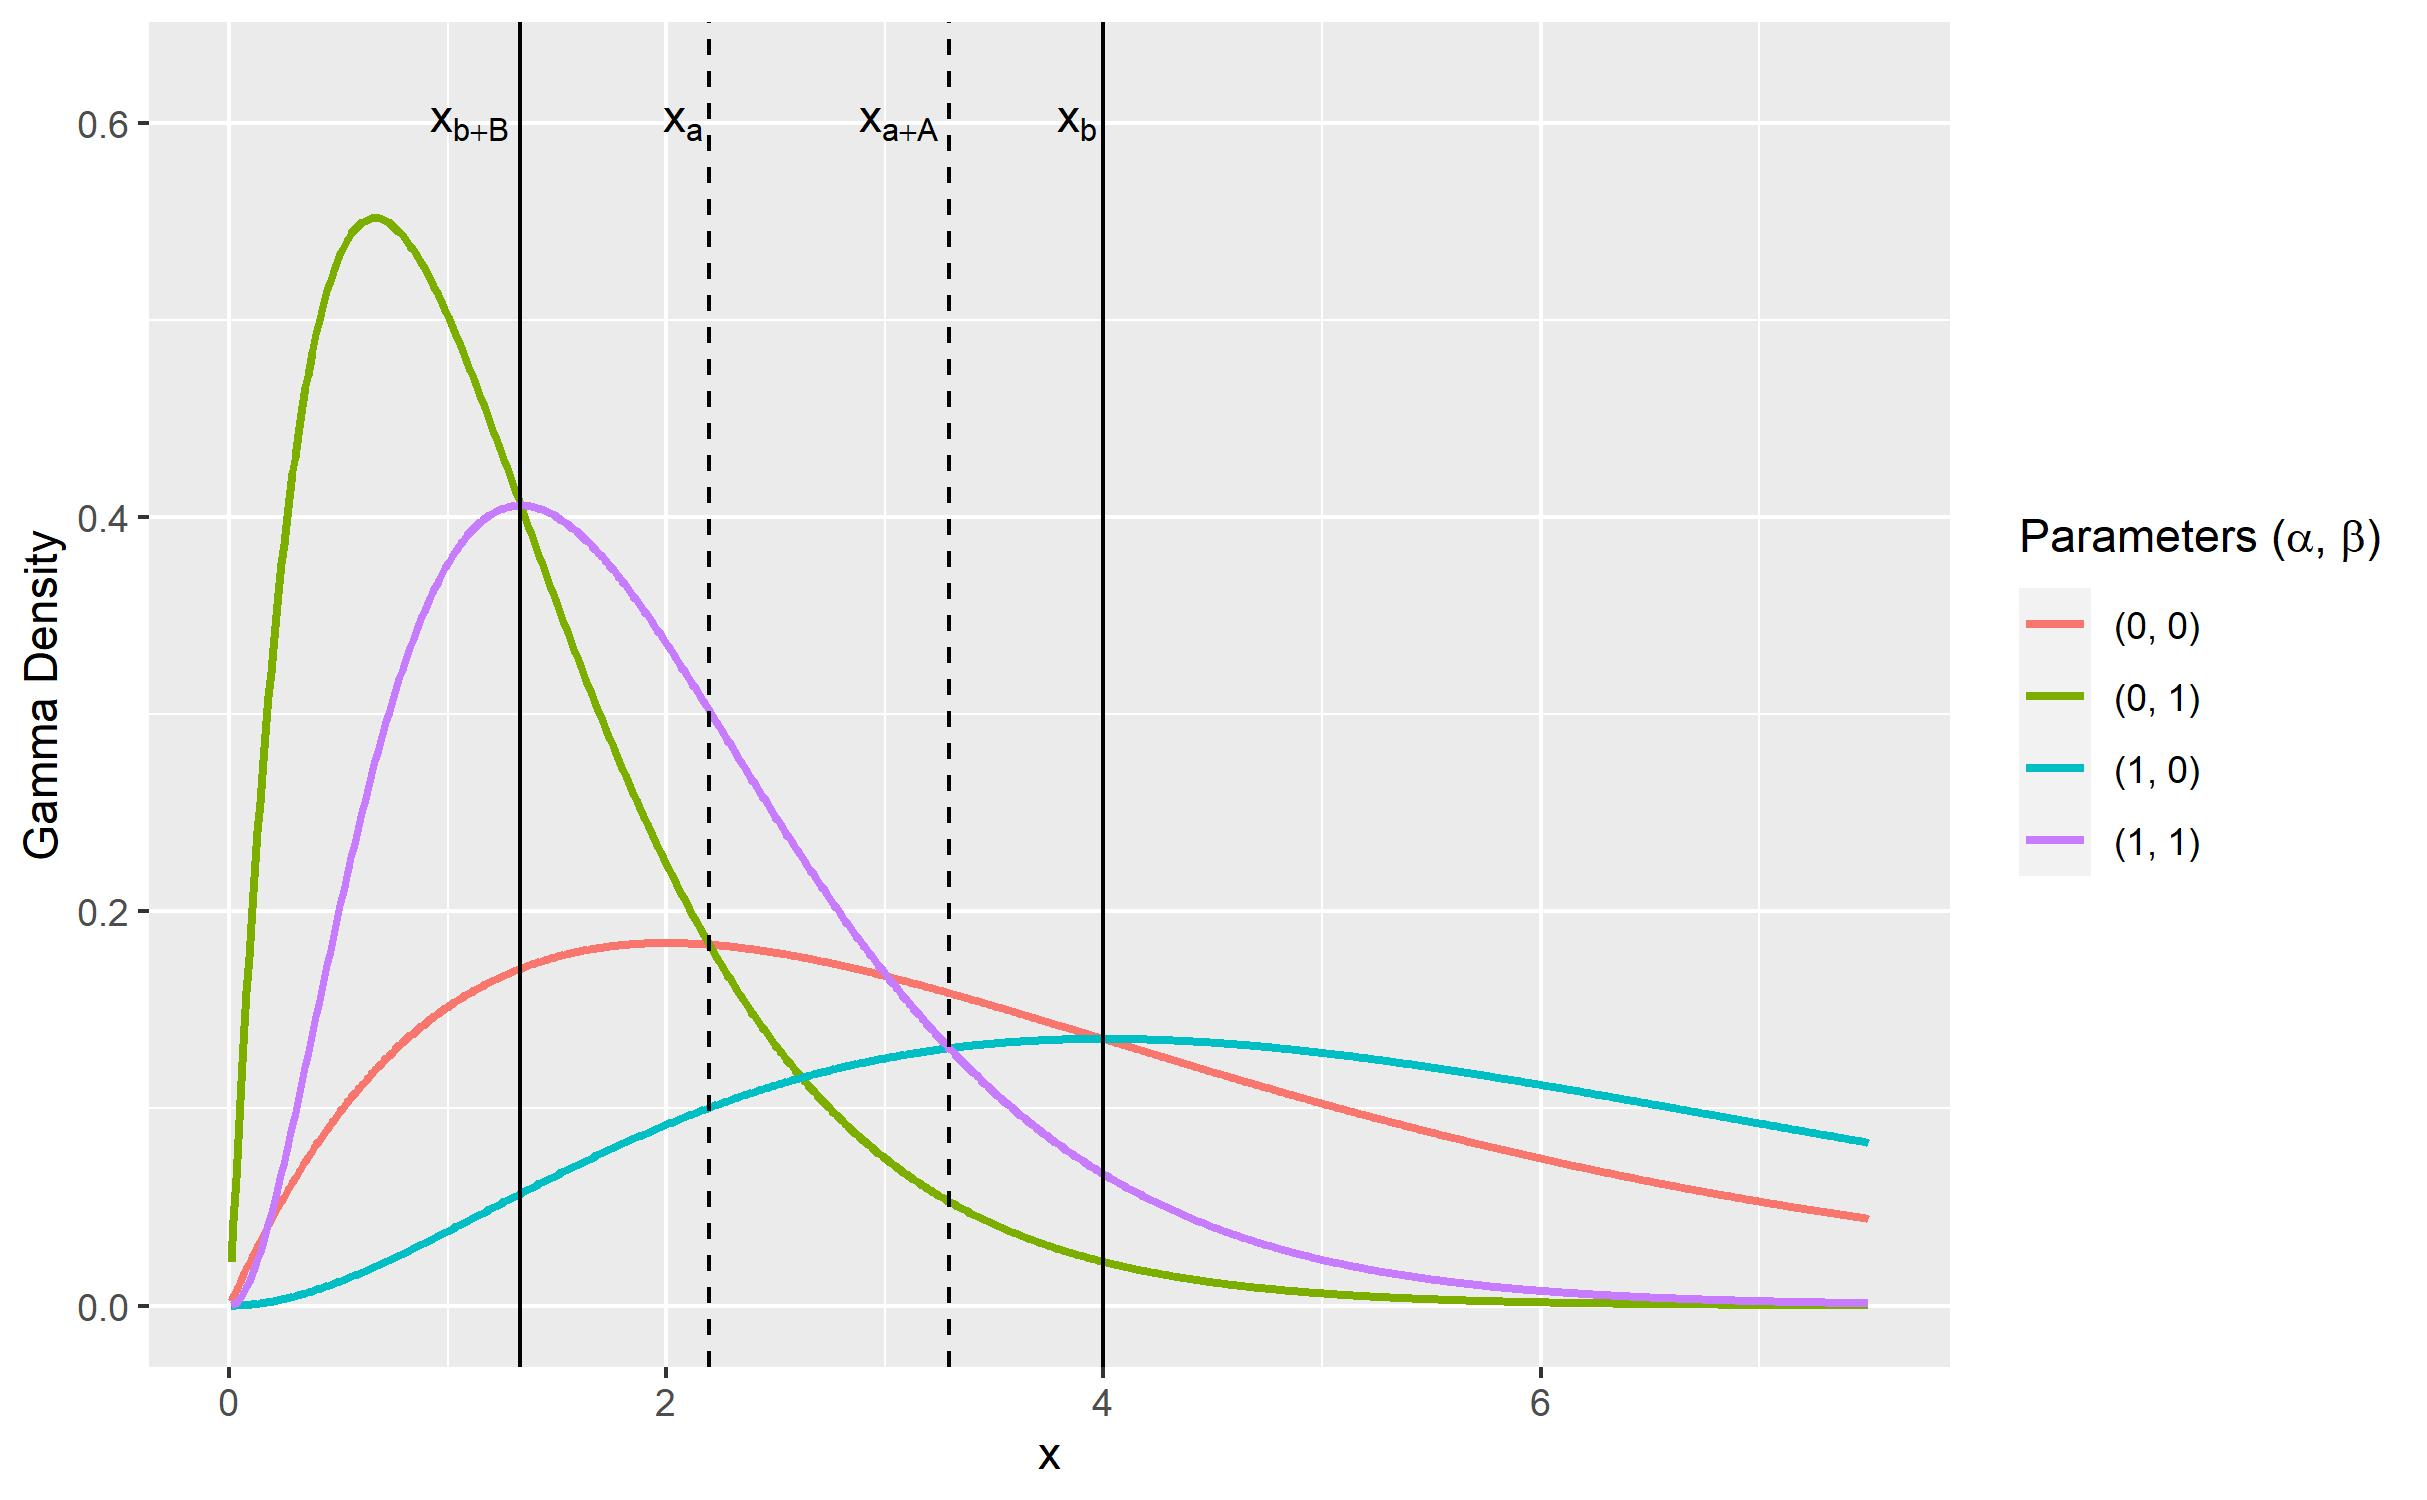
\includegraphics[width=\textwidth]{gamma_minorization_2.jpg}
	\caption{Example of minorization of the density of a gamma distribution $Ga(2+\alpha, 0.5+\beta)$ for $\alpha$ and $\beta$ jointly.}
	\label{fig:gam2}
\end{figure}

% Truncated Exponential
\begin{lemma}
	\label{pro:tru}
	$$\min_{0 \le \mu \le M} \TruncExp(u; \mu, 0, u) = \TruncExp(u; M, 0, u) $$
\end{lemma}
\begin{proof}
	Remember that $\TruncExp(u; \mu, 0, u) = \frac{\mu \exp\{-u\mu\}}{1-\exp\{-u\mu\}}$ is the density of an exponential distribution bounded above by $u$.
	\begin{align*}
		\frac{d}{d\mu}\TruncExp(u; \mu, 0, u)
		& = \left(\frac{\exp\{-u\mu\}}{1-\exp\{-u\mu\}} \right) \left[ 1-\mu u - \mu u \left(\frac{\exp\{-u\mu\}}{1-\exp\{-u\mu\}} \right) \right]
	\end{align*}
	Now let $g(\mu) = 1-\mu u - \mu u \left(\frac{\exp\{-u\mu\}}{1-\exp\{-u\mu\}} \right)$. By L'H\^{o}pital's rule, $g(0) = 0$. Moreover, for $\mu>0$, we have
	\begin{align*}
		g'(\mu)
		& = - \mu \left(1+\frac{\exp\{-u\mu\}}{1-\exp\{-u\mu\}} \right) \left[ 1-u\mu \left(\frac{\exp\{-u\mu\}}{1-\exp\{-u\mu\}} \right) \right]  \\
		& = - \mu \left(1+\frac{\exp\{-u\mu\}}{1-\exp\{-u\mu\}} \right) \left[ 1- \frac{u\mu}{\exp\{u\mu\}-1} \right] \\
		& \le 0
	\end{align*}
	where the inequality follows from $\frac{u\mu}{\exp\{u\mu\}-1}\le1$.
	This implies that $g(\mu) \le 0$ for $\mu>0$. We therefore have $\frac{d}{d\mu}\TruncExp(u; \mu, 0, u) \le 0$ and the result of the proposition follows.
\end{proof}


% Uniform Ergodicity
\begin{proposition}
	\label{pro:uni}
	The transition kernel $P = P_{\theta}P_{\z}$ satisfies a minorization condition $M(1, \delta, \chi, \nu)$ and is therefore uniformly ergodic.
\end{proposition}

\begin{proof}
	First, note that the transition kernel $P$ of our Markov chain is a composition of two kernels
	$$ P = P_{\theta} P_{\z}$$
	where the kernel $ P_{\theta}$ updates the parameters $\theta$ of $\x$ while keeping the augmented data $\z$ fixed and $P_{\z}$ update $\z$ while keeping $\theta$ fixed. A one-step transition therefore corresponds to the following scheme 
	$$\x_1 = (\theta_1, \z_1) \rightarrow (\theta_2, \z_1) \rightarrow (\theta_2, \z_2) = \x_2.$$
		
	The kernel $P$ has a density $p$ with respect to the product measure $\mu = \lambda \mu_{\z}$ with $\lambda$ the Lebesgue measure on $\chi_{\theta}$, the space of $\theta$, and $\mu_{\z}$ a $\sigma$-finite measure on $\chi_{\z}$, the space of $\z$.
	\begin{align*}
		P(\x_1, d\x_2) 
		& = p(\x_1, \x_2) \mu(d\x_2) \\
		& = p((\theta_1, \z_1), (\theta_2, \z_2)) \lambda(d\theta_2)\mu_{\z}(d\z_2) \\
		& = p_{\theta}((\theta_1, \z_1), (\theta_2, \z_1)) p_{\z}((\theta_2, \z_1), (\theta_2, \z_2)) \mu_{\z}(d\z_2) \lambda(d\theta_2)
	\end{align*}
	where
	\begin{align*}
		p_{\theta}((\theta_1, \z_1), (\theta_2, \z_1))
		& = q_{\theta}((\theta_1, \z_1), (\theta_2, \z_1)) \alpha((\theta_1, \z_1), (\theta_2, \z_1)) \\
		& = \pi(\theta_2| \z_1)
	\end{align*}
	is the density of the transition kernel $P_{\theta}$ with respect to $\lambda$ and corresponds to the full conditional distribution $\pi(\theta_2| \z_1)$ since the kernel $P_{\theta}$ is a Gibbs sampler, and
	\begin{align*}
		p_{\z}((\theta_2, \z_1), (\theta_2, \z_2))
		& = q_{\z}((\theta_2, \z_1), (\theta_2, \z_2)) \alpha((\theta_2, \z_1), (\theta_2, \z_2)) \\
		& = g(\z_2; \theta_2) \min\left\lbrace 1, \dfrac{\pi(\theta_2, \z_2)g(\z_1; \theta_2)}{\pi(\theta_2, \z_1)g(\z_2; \theta_2)} \right\rbrace \\
		& = \min\left\lbrace g(\z_2; \theta_2), \dfrac{\pi(\theta_2, \z_2)g(\z_1; \theta_2)}{\pi(\theta_2, \z_1)} \right\rbrace
	\end{align*}
	is the density of the transition kernel $P_{\z}$ with respect to $\mu_{\z}$ and corresponds to one step of the Metropolis-Hasting algorithm where a new specification of the augmented data $\z_2$ is proposed conditionally on the current value of the parameters $\theta_2$, but independently of the current specification of the augmented data $\z_1$.
	
	To show that $\chi$ is a small state, it is sufficient to show that there exists a function $k$ such that
	$$p(\x_1, \x_2) \ge k(\x_2) > 0, \qquad \forall \x_1 \in \chi $$
	for all $\x_2 \in \chi$.
	Note that the density $p$ is a function of $\x_1 = (\theta_1, \z_1)$ only through the full conditional distribution $\pi(\theta_2| \z_1)$ and the proposal density $g(\z_1; \theta_2)$.
	\begin{align*}
		p((\theta_1, \z_1), (\theta_2, \z_2))
		& = \min\left\lbrace \pi(\theta_2| \z_1)g(\z_2; \theta_2), \dfrac{\pi(\theta_2| \z_1) \pi(\theta_2, \z_2)}{\pi(\theta_2, \z_1)} g(\z_1; \theta_2) \right\rbrace \\
		& = \min\left\lbrace \pi(\theta_2| \z_1)g(\z_2; \theta_2),
		\dfrac{
			\frac{f(\theta_2, \z_1, Y)}{f(\z_1, Y)}
			\frac{f(\theta_2, \z_2, Y)}{f(Y)}
		}{\frac{f(\theta_2, \z_1, Y)}{f(Y)}} 
		g(\z_1; \theta_2)\right\rbrace \\
		& = \min\left\lbrace \pi(\theta_2| \z_1)g(\z_2; \theta_2),
		\dfrac{f(\theta_2, \z_2, Y)}{f(\z_1, Y)}
		g(\z_1; \theta_2)\right\rbrace \\
		& = \min\left\lbrace \pi(\theta_2| \z_1)g(\z_2; \theta_2),
		\pi(\theta_2| \z_2)
		g(\z_1; \theta_2)\right\rbrace
	\end{align*}
It therefore suffices to show that there exist functions $k_1$ and $k_2$ such that
$$\pi(\theta| \z_1) \ge k_1(\theta) > 0 \qquad \text{and} \qquad  g(\z_1; \theta) \ge k_2(\theta) > 0.$$

	First, 
	\begin{align*}
		\pi(\theta| \z_1) 
		& = \pi(\beta| \z_1) \pi(\gamma| \z_1)  \\
		& = Ga(\beta; a_{\beta} + n_T, b_{\beta} + SI_1) Ga(\gamma; a_{\gamma} + {n_J}_1, b_{\gamma} + I_1) \\
		& \ge h_{\beta}(\beta) h_{\gamma}(\gamma) \\
		& = k_1(\theta) > 0
	\end{align*}
	where, by Proposition \ref{pro:ga1},
	$$h_{\beta}(\beta) = \begin{cases}
		Ga(\beta;a_{\beta}+n_T,b_{\beta}), & \beta<\frac{a_{\beta}+n_T}{t_{end}(n_T+I_0) n} \log \left( 1 + \frac{t_{end}(n_T+I_0) n}{b_{\beta}}\right) \\ Ga(x;a_{\beta}+n_T,b_{\beta}+n(n_T+I_0) t_{end}), & \text{else}
	\end{cases}$$
since $n_T = \sum_k T_k$ is known and 
$$SI_1 = \int_{0}^{t_{end}}S_1(t)I_1(t)dt \in [0, n (n_T+I_0) t_{end}];$$
and, by Proposition \ref{pro:ga2},
	$$h_{\gamma}(\gamma) = \min\{
		Ga(\gamma;a_{\gamma}+n_T+I_0,b_{\gamma}), Ga(x;a_{\gamma},b_{\gamma}+(n_T+I_0) t_{end})\}
		$$
since $0\le n_1^J \le n_T + I_0$ and
$$I_1 = \int_{0}^{t_{end}}I_1(t)dt \in [0, (n_T+I_0) t_{end}].$$
	
	Second, each factor in
	\begin{align*}
		& g(\z_1; \theta) = \prod_{i=1}^{n_T} \TruncExp(z^T_i; \beta I_k, t_{k(i)-1}, t_{k(i)}) (1-p_i)^{1\{\z^J_i = \infty\}} (p_i \TruncExp(z^J_i; \gamma, z^T_i, t_{end}))^{1\{\z^J_i \le t_{end}\}}
	\end{align*}
	can be minorized as follows. First,
	\begin{align*}
		\TruncExp(z^T_i; \beta I_k, t_{k(i)-1}, t_{k(i)}) 
		& \ge \TruncExp(t_{k(i)}; \beta I_k, t_{k(i)-1}, t_{k(i)}) \\
		& \ge \TruncExp(t_{k(i)}; \beta (n_T + I_0), t_{k(i)-1}, t_{k(i)}),
	\end{align*}
	with the last inequality following from proposition \ref{pro:tru}, second,
	$$1-p_i = \exp\{-\gamma (t_{end} - z^T_i)\} \ge \exp\{-\gamma (t_{end} - t_{k(i)-1})\},$$
	third,
	$$p_i \TruncExp(z^J_i; \gamma, z^T_i, t_{end}) = \Exp(z^J_i - z^T_i; \gamma)1(z^T_i < z^J_i \le t_{end}) \ge \Exp(t_{end} - t_{k(i) - 1}; \gamma)$$
	where the equality holds since $p_i = P(z^J_i \le t_{end}|z^J_i > z^T_i)$ is equal to the normalizing constant of the truncated exponential.
	
	Taken together, these inequalities give
	\begin{align*}
		g(\z_1; \theta)
		& \ge \prod_{i=1}^{n_T} \TruncExp(t_{k(i)}; \beta (I_0 + n_T), t_{k(i)-1}, t_{k(i)}) \min\{\exp\{-\gamma (t_{end} - t_{k(i) - 1})\}, \Exp(t_{end} - t_{k(i) - 1}; \gamma)\} \\
		& = k_2(\theta) > 0
	\end{align*}
	which completes the proof.
\end{proof}
			
	\bibliographystyle{plain}
	\bibliography{bibliography}
		
\end{document}